% !TEX encoding = UTF-8 Unicode
% !TEX spellcheck = en-US


% This is the root file of your thesis: thesis.tex
% A line starting with % is a comment. In some cases, I have included a command preceded by a %. You may activate the command by removing the %.

%%===================================
\documentclass[12pt]{report}
\usepackage{ramsstyle}
\usepackage{pdfpages}
\usepackage{float}
\usepackage{hyperref}
\usepackage{mathtools}
\usepackage{array}
\usepackage{booktabs}

\setlength{\heavyrulewidth}{1.5pt}

\newcommand*{\fullref}[1]{\hyperref[{#1}]{\ref*{#1} \nameref*{#1}}} % One single link

\restylefloat{table}
%%===================================
%Write the various parts of your thesis as separate files and include them into the main file by the command \include{name of included file}. When you compile the LaTeX file, you may choose which subfiles to include by the command

%\includeonly{chapter01,chapter02}

%%===================================
\begin{document}
% !TEX encoding = UTF-8 Unicode
%!TEX root = thesis.tex
% !TEX spellcheck = en-US

%This is the Titlepage
%%=========================================
\thispagestyle{empty}

\includegraphics[scale=1.1]{fig/NTNU}
\mbox{}\\[6pc]
\begin{center}
\Huge{Energy Efficiency Experiments on Exynos 5 using OmpSs}\\[2pc]

\Large{Rune Holmgren}\\[1pc]
\large{December 2014}\\[2pc]

PILOT PROJECT FOR MASTER THESIS\\
Department of Computer and Information Science\\
Norwegian University of Science and Technology
\end{center}
\vfill

\noindent Supervisor 1: Professor Lasse Natvig

\noindent Co supervisor: Antonio Garcia Guirado

 % This is the titlepage
\setcounter{page}{0}
\pagenumbering{roman}
%% !TEX encoding = UTF-8 Unicode
%!TEX root = thesis.tex
% !TEX spellcheck = en-US
%%=========================================
\addcontentsline{toc}{section}{Preface}
\section*{Preface}
Here, you give a brief introduction to your work. What it is (e.g., a Master's thesis in RAMS at NTNU as part of the study program xxx and\ldots), when it was carried out (e.g., during the autumn semester of 2021). If the project has been carried out for a company, you should mention this and also describe the cooperation with the company. You may also describe how the idea to the project was brought up.

You should also specify the assumed background of the readers of this report (who are you writing for).\\[2cm]

\begin{center}
Trondheim, 2012-12-16\\[1pc]
(Your signature)\\[1pc]
Ola Nordmann
\end{center}

%% !TEX encoding = UTF-8 Unicode
%!TEX root = thesis.tex
% !TEX spellcheck = en-US
%%=========================================
\addcontentsline{toc}{section}{Acknowledgment}
\section*{Acknowledgment}
I would like to thank the following persons for their great help during \ldots

If the project has been carried out in cooperation with an external partner (e.g., a company), you should acknowledge the contribution and give thanks to the involved persons.

You should also acknowledge the contributions made by your supervisor(s).

\begin{flushright}
O.N.\\[1pc]
(Your initials)
\end{flushright}

%% !TEX encoding = UTF-8 Unicode
%!TEX root = thesis.tex
% !TEX spellcheck = en-US
%%=========================================
\addcontentsline{toc}{section}{Summary and Conclusions}
\section*{Summary and Conclusions}
Here you give a summary of your your work and your results. This is like a management summary and should be written in a clear and easy language, without many difficult terms and without abbreviations. Everything you present here must be treated in more detail in the main report. You should not give any references to the report in the summary -- just explain what you have done and what you have found out. The Summary and Conclusions should be no more than two pages.

You may assume that you have got three minutes to present to the Rector of NTNU  what you have done and what you have found out as part of your thesis. (He is an intelligent person, but does not know much about your field of expertise.)
% !TEX encoding = UTF-8 Unicode
%!TEX root = thesis.tex
% !TEX spellcheck = en-US
%%=========================================
\addcontentsline{toc}{section}{Problem statement}
\section*{Problem statement}
The report is the pilot project for my planned master thesis in the spring of 2015.
The goal of the project is to present preliminary experiment data about the energy efficiency of the Exynos 5 using OmpSs.
The experiments should unveil the potential of task based programming on the Exynos 5.
They should also explore the ARM big.LITTLE architecture, and discuss how well suited task based programming is to achieve parallelism on heterogeneous platforms.

Another important purpose of this project, is to get familiar with the OmpSs system and experiment platforms.
Extensive deep digging experiments does not fit within the scope of this project, and it is more important that the research lay down a foundation for future work.

% !TEX encoding = UTF-8 Unicode
%!TEX root = thesis.tex
% !TEX spellcheck = en-US
%%=========================================
\addcontentsline{toc}{section}{Acknowledgements}
\section*{Acknowledgments}
I would like to thank my supervisor Professor Lasse Natvig, who has been guiding me during the last months.
I would also like to thank my co-supervisor PhD Antonio Garcia Guirado, who has been helping me with all small and large problems that have come up during the research.
They have both been enthusiastically following my work, and continuously guiding me and supplying me with valuable feedback.
I am sincerely thankful for all their help.

% !TEX encoding = UTF-8 Unicode
%!TEX root = thesis.tex
% !TEX spellcheck = en-US
%%=========================================
\addcontentsline{toc}{section}{Abstract}
\section*{Abstract}
This is the abstract.

\tableofcontents
\setcounter{page}{0}
\pagenumbering{arabic}
% !TEX encoding = UTF-8 Unicode
%!TEX root = thesis.tex
% !TEX spellcheck = en-US
\chapter[Introduction]{Introduction}
\section{Motivation}
Increase of performance and power efficiency are the main goal of processor designers.
Unfortunately we are currently reaching the limits of our current techniques.
For some time, hardware developers have been struggling to achieve increased performance.
Heat prevent us from driving the clock frequencies higher, while memory performance is lagging more and more behind.
A solution to enable continued performance growth is multi core processors, and for the last decade this has been the focus of research.
Unfortunately adding cores will not be a sustainable solution forever.
As the amount of cores grow, they are still competing for the same system resources and may have to wait for each other to complete calculations on data with dependencies \cite{hill07}.

A promising solution to this issue is heterogeneous multi-processor systems.
Heterogeneous multi-processor systems utilize multiple different processor cores in the same system.
This allow different parts of a program to be executed on a suitable processor.
By using a suitable core for each part of the program it is possible to achieve better performance and energy efficiency than homogeneous multi-processor systems \cite{kumar03}.
Programming of such systems is challenging, as it require manual labor to adapt the system for different processors. 
Task based programming may be a solution, as it allow the programmer to write the tasks in a general manner, leaving the scheduler to distribute the tasks.

\section{Project Scope and Goal}
This pilot projects main goal is to do preliminary research and experiments on the energy efficiency of the Exynos 5 processor, with the intent to use the results next spring in my master thesis.
The goal of this research is to explore the potential of the task based programming model on heterogeneous multi-processor systems.

\section{Problem Statement Interpretation and Approach}
\begin{itemize}
  \item Task 1: Get the OmpSs task based programming model framework running on both test platforms.
  \item Task 2: Implement or adapt a suitable experiment application for testing energy efficiency.
  \item Task 3: Implement some energy efficiency measurement application for ODROID-XU3.
  \item Task 4: Optimize experiment applications for both platforms.
  \item Task 5: Gather performance and energy efficiency results from the experiment applications on both platforms.
  \item Task 6: Analyze, present and discuss experiment results.
\end{itemize}

\subsubsection{Task 1}
This project will present results on programs utilizing task based programming.
It is essential to get the OmpSs framework, which will be used in the experiments, running on both test platforms.
This task should be solved before progressing any further, as any issues here would render further work useless.

\subsubsection{Task 2}
To be able to determine anything about the potency of the task based programming model on our test platforms, we need a test application.
The application should be suitable for the parallel environment of our test platforms, and include some kind of performance metric.
The purpose of developing or adapting such an application is to have a way of gathering data about the platform.
As a result of this, it is not important what the application does, as long as it does something meaningful.

\subsubsection{Task 3}
The ODROID-XU3 include current and voltage sensors.
Recording data from these sensors during experiment execution will be the source of energy metrics.
A software solution to gather these data will have to be implemented before any of the data necessary for the rest of the project can be gathered.

\subsubsection{Task 4}
Parallel applications will always behave different on different platforms.
It is possible to manually tune such applications to specific platforms.
This is work that can be done very thoroughly, but this is time consuming work that is not the main goal of this project.
There should at least be made an effort to make some optimizations to the applications, to ensure that they are performing well on the test platforms.

\subsubsection{Task 5}
When all preceding steps are completed, it is time to gather data.
The application from task 2 should be tuned with the optimizations from task 4.
Then it should be executed with the energy measurements tool from task 3.
The resulting data should hopefully contain interesting information to discuss.

\subsubsection{Task 6}
The data from the application should be analyzed.
The focus of this analysis should be the energy efficiency with attention to trade off against performance.
It is interesting to see how the different test platforms and configurations perform compared to each other.
There will be many comparisons to make here.
The promising results should be elaborated, and their potential discussed.

\section{Outline}
This is the outline of the report, explaining what each part of it contains.

\subsubsection{Introduction}
In the introduction chapter, the report and it's purpose are introduced.
The motivation of the paper is presented, together with its goal.
There is also an explanation of how the problem was interpreted and approached.

\subsubsection{Background}
In the background chapter, existing theory and related work is presented.
Most of the general concepts necessary to understand the rest of the project is presented briefly.
The main areas explained are energy efficiency and measurements, vector instructions, the task based programming model and heterogeneous multi-processors.
In addition, the experiments used in the paper and the platforms they were run on are introduced.

\subsubsection{Setup and methodology}
In the setup and methodology chapter, the technical details about how the experiments were run are explained.
This includes listings of software used, with version numbers and details on how it was used, including flags used for experiment compilation.
There are also explanations about how performance and energy efficiency measurement were gathered.

\subsubsection{Results and discussion}
In this chapter the results of the experiments are presented and discussed.
The experiments presented are covering optimizations, performance, and power and energy measurements.
The discussion elaborates what the results mean for the potential of task based programming on heterogeneous multi-processors.

\subsubsection{Conclusion}
In this chapter the conclusions we are able to draw from the discussions are presented.
Central here are the results indicating the potential of task based programming on heterogeneous multi-processors.

\subsubsection{Future work}
In the future work chapter, the unexplored aspects of the research are presented.
There are a lot of tasks that were not included in this project's scope, as this was a pilot project.
Many of these tasks will hopefully be addressed in the planned master thesis built on what was learned from this project.
These tasks are presented in this chapter.


% !TEX encoding = UTF-8 Unicode
%!TEX root = thesis.tex
% !TEX spellcheck = en-US
\chapter[Related work]{Related work}


%!TEX root = thesis.tex
% !TEX spellcheck = en-US
\chapter[Background]{Background}

\section{Energy efficiency} \label{energymeasurement}
Computers consume energy.
Achieving low energy consumption is an area of great interest, both in super computers where power is expensive and in consumer hardware where low power mean longer battery life.
The energy consumption of a system depend both on hardware and software.
The hardware of the system will typically run within a narrow range of voltages, and the components of the system have some current drag when they are working.
The programmer can not affect how large these values are.
What can be done however, is to ensure that the software does not consume energy unnecessary.
The some of the components in the system that are not used can be turned off.
Some of the features of a processor may also cause it to consume more power.
An example is NEON vector instructions, which have been shown to increase the power usage of the system by up to 20\%\cite{TrondIngeLillesand} when used.
Turning off components or features does save power, but there will often be a performance loss.
When energy efficiency is a goal, there is always questions about how much power can be saved before the execution time is extended so much that there is a total loss in power consumed.
Because of this, it is interesting to analyze programs with regard to energy consumption.

\subsubsection{Energy measurement}
There as mentioned, the interesting power properties of a system is voltage and current.
In systems featuring sensors for such data, the data can be gathered while executing a program.
By analyzing the data it is possible to optimize the program for energy efficiency.

The power of the system is the product of the voltage and current.
This is interesting to observe in applications that run when the system is standing by.
When execution time doesn't matter, the energy consumed per time is what matter.

Often the system is executing a program for a duration, and as soon as it is done the system can be shut down.
In such cases it is interesting to measure how much energy the system consumed during execution.
The product of the systems power and the problems execution time, is the total amount of energy consumed.

There are many cases where a balance between energy efficiency and the performance trade off is interesting.
This is when the energy delay product of the system become interesting.
This is valid both for scientific experiments and programs executed on regular systems.
In research experiments the goal may be to obtain energy efficiency or performance.
In either case, it is sensible to remember that the actual goal will normally be a balance between the two.
On regular systems in real life applications, both energy and performance matter.
Users does not want to wait longer than necessary for the system to complete its task.
Neither do they want the system to run out of battery or the power bill to grow too big.
The energy delay product of a system is calculated by multiplying the execution time of the application with its energy.

\section{NEON}
NEON is a general-purpose single input multiple data (SIMD) technology implemented in the ARM Cortex-A series of processors.
It is able to run SIMD instructions on 128 bit registers.
By utilizing the NEON unit of the ARM processors, it is possible to achieve parallelism in each separate core.
This will often open for great performance boost on problems like the ones explored in this paper.
Each register may be filled with single precision floating point numbers ranging from 8 to 64 bit each.
This mean that the programmer may choose to fill them with 16 8 bit numbers, 8 16 bit numbers, 4 32 bit numbers, 2 64 bit numbers or a single 128 bit number.
This allow a single thread to achieve parallelism.
In future generations of the ARM ISA there will be support for other data types as well\cite{This need to be cited}.
Different implementations of NEON exist in the Cortex A cores, and while the even the simple implementations in smaller cores like the A7 can give great performance boost, the implementations present in the newest cores are performing even better.
The A15 offer two NEON units, and the instruction pipeline to start the cores are shorter than in simpler implementations.

\section{Task based programming}
Task based programming allow a programmer to work with parallel programs, with an abstraction from the parallelization itself.
When programming with this model, the program can be split into tasks which can run in parallel.
When the program run, it will run a task manager as part of the program.
This task manager can dynamically assign tasks to the processors, and the programmer does not have to handle all the time consuming tasks related to manual parallelization.
As long as the programmer correctly handle dependencies in the parallelized code, it will be possible to write this kind of code as if it was serial.

The task based programming model also allow simpler development of portable programs.
When the program is running tasks on available CPUs, it is not a problem to allow it to run on larger or smaller numbers of processors, and even clusters can support the program.
This model even allow the tasks to run on different types of processors in a heterogeneous environment.

\section[OmpSs]{OpenMP Super scalar}
OpenMP Super scalar (OmpSs) is a extension of the OpenMP API to integrate features from the StarSs programming model.
It is currently under development at the Barcelona Supercomputing Center.
The goal of OmpSs is to extend the programming model to support a wide range of processors.
The OmpSs programming model will run on a wide variety of different systems, such as traditional personal computers, clusters, shared memory systems and heterogeneous processors.
While the software is not yet completed or fully tested, there have been several reports exploring it's potential.
The results have proven OmpSs as an efficient solution on both clusters and heterogeneous systems utilizing OpenCL and CUDA.


\section{Heterogeneous multi-processor}
Heterogeneous multi-processor systems have multiple different processors, opposed to traditional multi-processor systems.
A typical modern processor have several processors, and a program can run effectively by having threads running parts of thesis work on each of them.
This work is often of such a nature that it can run better on a different processor.
Sometimes it can run just as well on multiple simple processor, while using less die space and energy.
In other instances, an advanced processor with some special capabilities, like vector instructions, can be more efficient.

  This kind of processors have a potential to help us overcome the challenges that are emerging in processor development.
    Unfortunately they also introduce several new challenges.

\section{Experiment platforms}

\subsection{Arndale Board} \label{ArndaleBoard}
\begin{figure}[ht!]
  \centering
  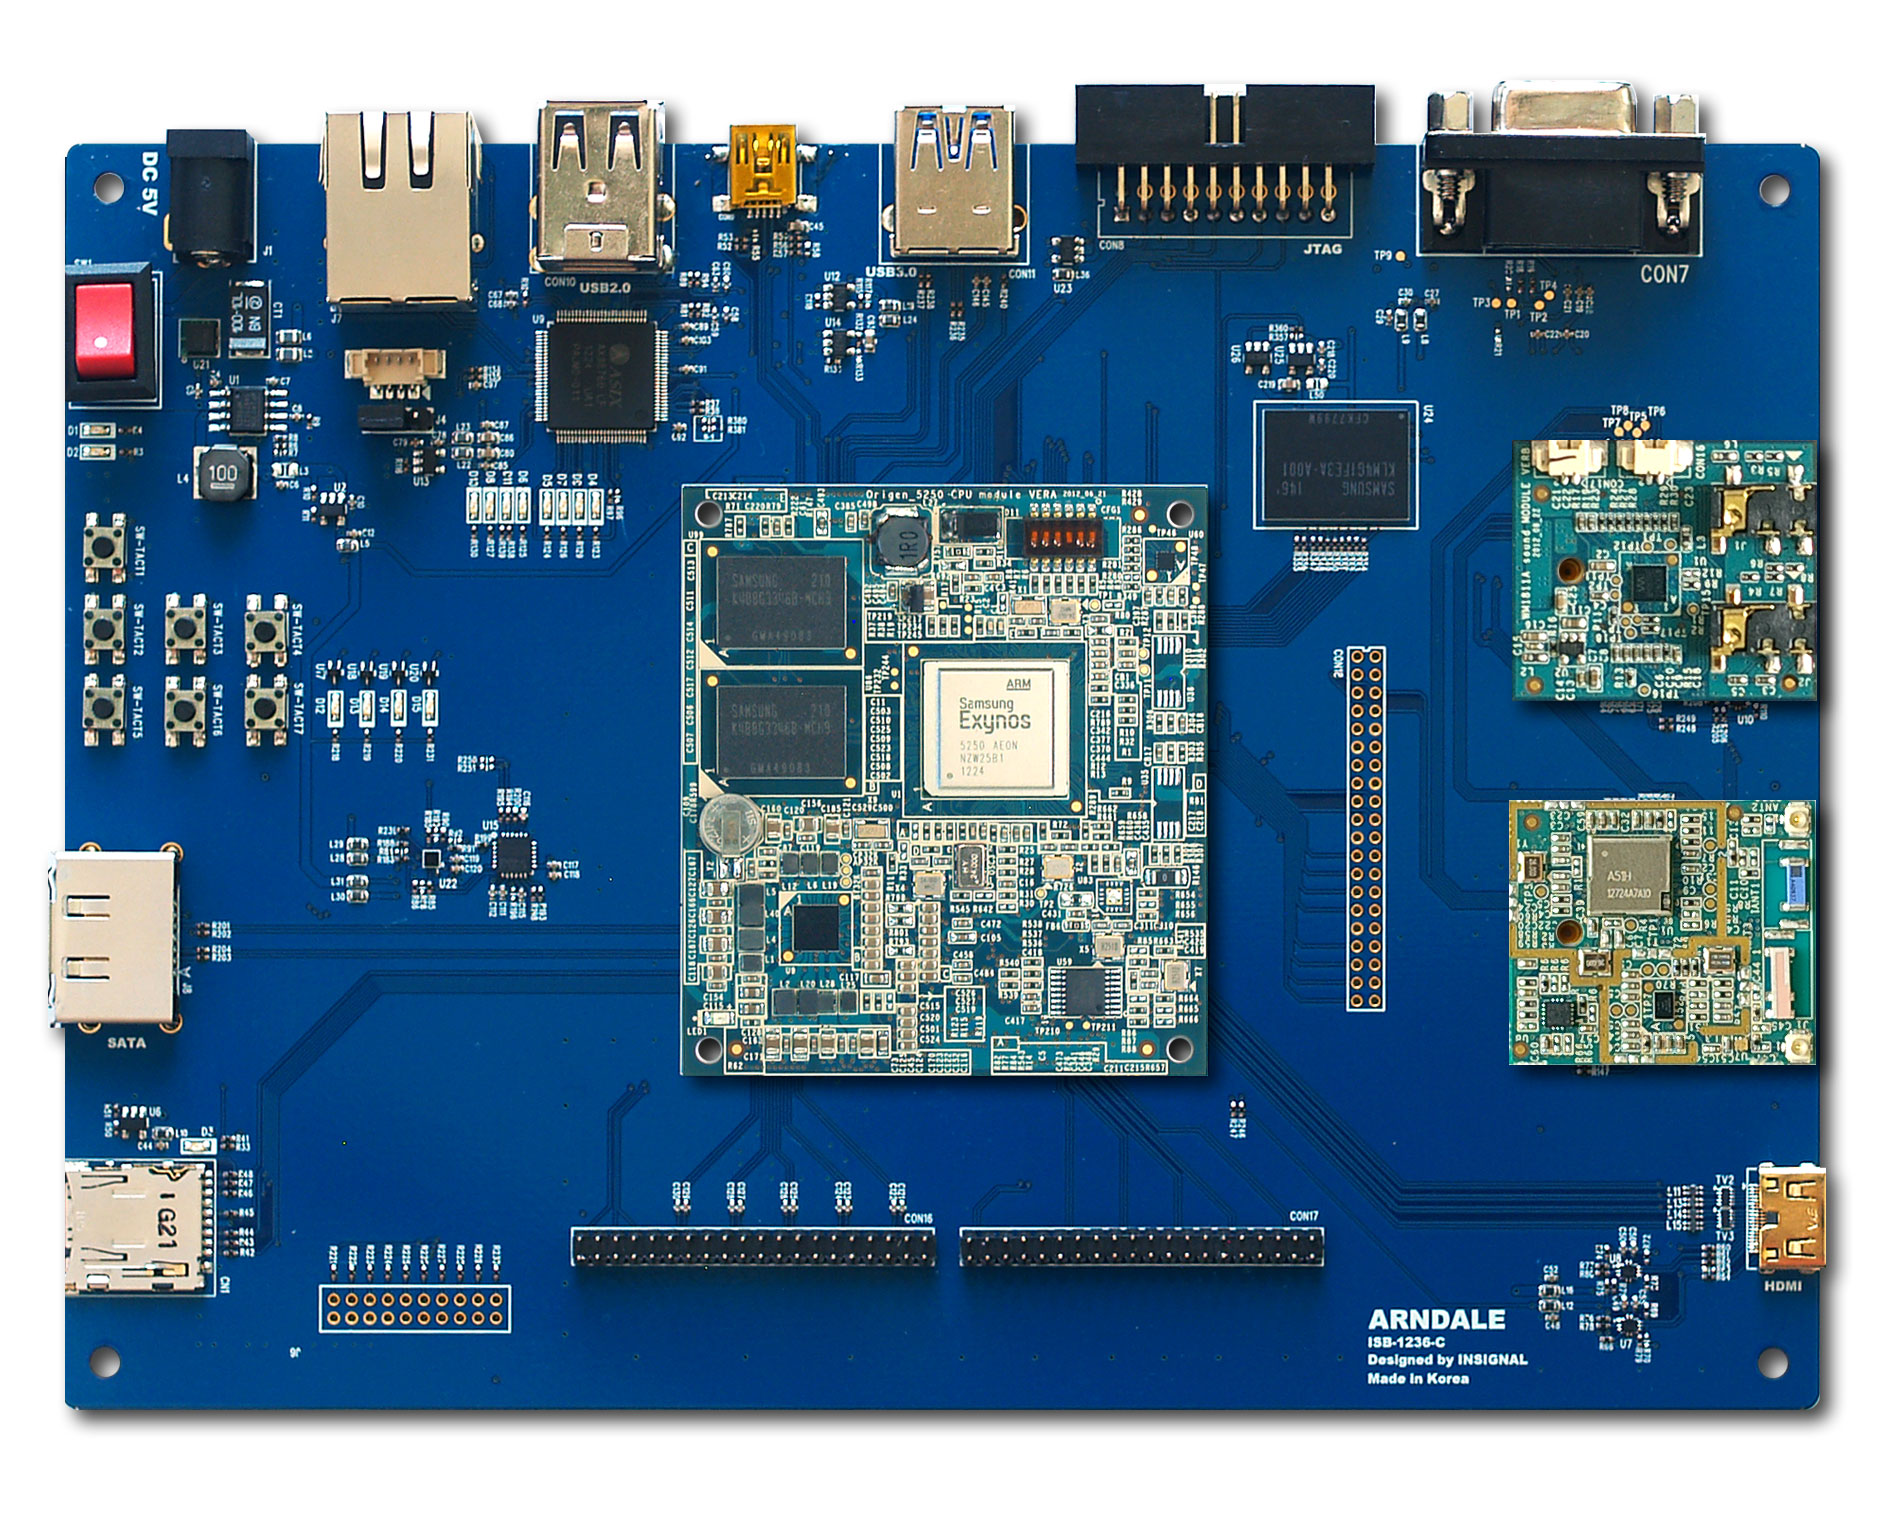
\includegraphics[width=90mm]{fig/Arendale.jpg}
  \caption{Arndale Duo \label{overflow}}
\end{figure}
The Arndale Duo is a computing system mounted on a single board.
It is fitted with an Exynos 5250 SoC, which contain a dual core ARM Cortex-A15 , as well as an ARM Mali T-604 GPU.
This computer offer a range of supported Linux distributions, as well as the OmpSs programming model.
The Arndale Duo board was used for some preliminary research in this thesis.
It was chosen because we had experience from earlier student projects using this board.
The computer was used in the 2014 master thesis "Acceleration with OmpSs and Neon/OpenCL on ARM Processor" by Trond Inge Lillesand.
The thesis lay a lot of the ground for this pilot project and planned master thesis.

\begin{table}[h]
  \begin{tabular}{ll}
    \toprule
    \textbf{SoC}              & Samsung Exynos 5250 \\
    \midrule
    \textbf{CPU}              &  \\
    Model                     & ARM Cortex-A15 \\
    Manufacturing process     & 32nm \\
    Maximum clock frequency   & 1.7GHz \\
    Number of cores           & 2 \\
    L2 Cache                  & 1MB \\
    L1 Cache                  & 32KB \\
    \midrule
    \textbf{GPU}              &  \\
    Model                     & ARM Mali-T604 \\
    Maximum clock frequency   & 600 MHz \\
    Number of cores           & 4 \\
    \midrule
    \textbf{Memory}           &  \\
    Available memory          & 2 GB \\
    Maximum clock frequency   & 800MHz \\
    \midrule
    \textbf{Operating system} &  \\
    Distribution              & Linux Ubuntu \\
    %Version                   & TODO \\
    \bottomrule
  \end{tabular}
  \caption{Arndale Duo Specifications\label{overflow}}
\end{table}

\subsection{ODROID-XU3} \label{OdroidXU3}
\begin{figure}[H]
  \centering
  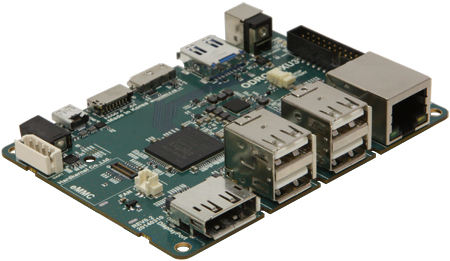
\includegraphics[width=90mm]{fig/ODROID.jpg}
  \caption{ODROID-XU3 \label{overflow}}
\end{figure}
The ODROID-XU3 is a new single-board computing system, offering interesting properties for these experiments.
The system has an Exynos 5422 heterogeneous SoC.
Exynos 5422 has a quad core ARM Cortex-A15 CPU and a ARM Mali T-628 GPU, but also a smaller quad core ARM Cortex-A7 processor.
These 3 different processing units can be used simultaneously to solve problems.
They use ARMs big.LITTLE architecture to achieve this heterogeneous system.
In this paper, and the planned master thesis following it, the potency of this kind of heterogeneous processor will be explored.
This is the system that will run most of the experiments, including all energy efficiency experiments.

\begin{table}[H]
  \begin{tabular}{ll}
    \toprule
    \textbf{SoC}              & Samsung Exynos 5422 \\
    \midrule
    \textbf{CPU 1}            &  \\
    Model                     & ARM Cortex-A15 \\
    Manufacturing process     & 32nm \\
    Maximum clock frequency   & 2.0GHz \\
    Number of cores           & 4 \\
    L2 Cache                  & 512KB \\
    L1 Cache                  & 32KB/32KB I/D \\
    \midrule
    \textbf{CPU 2}            &  \\
    Model                     & ARM Cortex-A7 \\
    Manufacturing process     & 32nm \\
    Maximum clock frequency   & 1.4GHz \\
    Number of cores           & 4 \\
    L2 Cache                  & 2MB \\
    L1 Cache                  & 32KB/32KB I/D \\
    \midrule
    \textbf{GPU}              &  \\
    Model                     & ARM Mali-T628 MP6 \\
    Maximum clock frequency   & 600 MHz \\
    Number of cores           & 4 \\
    \midrule
    \textbf{Memory}           &  \\
    Available memory          & 2 GB \\
    Maximum clock frequency   & 933MHz \\
    \midrule
    \textbf{Operating system} &  \\
    Distribution              & Linux odroid \\
    Version                   & 3.10.54+ \\
    \bottomrule
  \end{tabular}
  \caption{ODROID-XU3 Specifications\label{overflow}}
\end{table}

\subsubsection{Power monitoring}
The ODROID-XU3 comes with integrated power monitoring tools.
Implemented in hardware, it have got 4 current sensors sitting on the power pins of the Exynos SoC.
The energy monitors are indicated in figure \ref{overview-odroid}.
These monitor the current going through the large CPU cores, the small CPU cores, memory and GPU respectively.
In addition to the current sensors, the power management for the SoC is also available to the programmer, making supply voltage to the components known.
By using the voltage and current, the power consumption is known.
As a whole, the system offer frequency, voltage, current, temperature and power readings in real time.
These fine energy and performance metrics make the system highly suitable for developers.
They are able to run their programs, collect energy profiling data and optimize their software based on the result.

\begin{figure}[ht!]
  \centering
  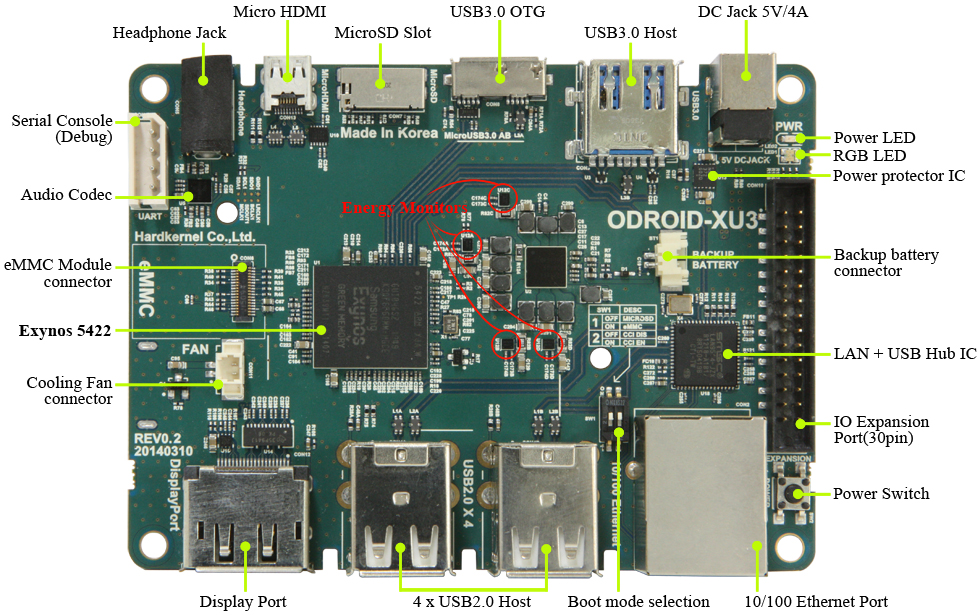
\includegraphics[width=130mm]{fig/overview-odroid.jpg}
  \caption{ODROID-XU3 annotated (hardkernel.com\cite{hardkernel01})\label{overview-odroid}}
\end{figure}

\subsubsection{Performance}

The ODROID-XU3 comes with the ARM Cortex-A15 limited to 2GHz and the ARM Cortex-A7 limited to 1.4GHz.
There is 2GB of memory available running at 800 MHz, and the ARM Mali T-628 GPU run at 600 MHz.
This performance place it at the higher end of SoCs, but not quite in the top, as it is beaten by systems like TODO A reference system here).
The ODROID-XU3 feature the new eMMC 5.0 standard for storage.
The performance of this standard outperform both older eMMC standards, as well as memory card readers, which other similar systems may contain.
The ODROID-XU3 can achieve a read/write performance of 198/74 MB/s\cite{hardkernel01}, which a lot better than older systems like the Arndale Duo.

In addition to the eight processor cores, the system also feature a ARM Mali T-628.
The Mali T-628 function both as a regular GPU, as well as a GPGPU.
It support both openGL and DirectX, and is able to produce graphics for all but the most demanding gaming and simulation purposes.
In addition to this it is able to run computations with Open CL.
This mean that problems with parallel parts, can be solved efficiently utilizing the GPU.

\subsection{ARM Cortex-A15}
The ARM Cortex-A15 is a high performance processor core designed for use in a wide range of applications from small embedded systems, to larger consumer electronics.
This processor core is present in both the Arndale Duo and the ODROID-XU3, who have 2 and 4 such cores respectively.
In the latter, 4 smaller ARM Cortex-A7 cores are also featured, and all can be used simultaneously.
\begin{table}[H]
  \begin{tabular}{ll}
    Frequency         & 1.0 GHz to 2.5GHz  \\
    L1 Cache          & 64KB \\
    L2 Cache          & 4 MB \\
    L3 Cache          & None in core, may be implemented shared in multi core system. \\Architecture      & ARMv7-A            \\
    Architecture      & ARMv7-A            \\
                      & TrustZone® security technology \\
                      & NEON™ Advanced SIMD \\
                      & DSP \& SIMD extensions \\
                      & VFPv4 Floating point \\
                      & Hardware vitalization support \\
                      & Integer Divide \\
                      & Fused MAC \\
                      & Hypervisor debug instructions \\
    Memory management & 40-bit ARMv7 Memory Management Unit
  \end{tabular}
\end{table}
\subsection{ARM Cortex-A7}
The ARM Cortex-A7 is designed to be a low power alternative to the ARM Cortex-A15 and ARM Cortex-A17, with the same supported ISA and features.
This enable the ARM Cortex to be paired with it's larger relatives in a ARM big.LITTLE configuration.
4 of these cores are featured in the Exynos 5422 SoC on the ODROID-XU3 board.
\begin{table}[H]
  \begin{tabular}{ll}
    Frequency         & 1.2 GHz to 1.6GHz  \\
    L1 Cache          & 8-64KB \\
    L2 Cache          & up to 1 MB \\
    L3 Cache          & None in core, may be implemented shared in multi core system. \\
    Architecture      & ARMv7-A            \\
    Supported features& ARM Thumb-2 \\
                      & TrustZone® security technology \\
                      & NEON™ Advanced SIMD \\
                      & DSP \& SIMD extensions \\
                      & VFPv4 Floating point \\
                      & Hardware vitalization support \\
                      & Integer Divide \\
                      & Fused MAC \\
                      & Hypervisor debug instructions \\
    Memory management & 40-bit ARMv7 Memory Management Unit
  \end{tabular}
\end{table}
\subsection{ARM Mali T604}
This is a high performance low power mobile GPU.
The Arndale Duo board feature one of these in it's Exynos 5250 SoC.
\begin{table}[H]
  \begin{tabular}{ll}
    Frequency         & 533 MHz\\
                      & 17 GFLOPS  \\
    Multi core support & 1-4 cores  \\
    API Support       & OpenGL 1.1, 2.0, 3.0 and 3.1  \\
                      & OpenCL 1.1  \\
                      & DirectX 11  \\
                      & RenderScript \\
    Anti-Aliasing     & 4xFSAA with minimal performance drop  \\
                      & 16xFSAA  \\
    Cache             & 32-256KB L2 cache
  \end{tabular}
\end{table}
\subsection{ARM Mali T628}
This is a high performance low power mobile GPU.
The ODROID-XU3 board feature one of these in it's Exynos 5244 SoC.
\begin{table}[H]
  \begin{tabular}{ll}
    Frequency         & 533/695 MHz \\
                      & 17/23.7 GFLOPS \\
    Multi core support & 1-8 cores  \\
    API Support       & OpenGL 1.1, 2.0, 3.0 and 3.1  \\
                      & OpenCL 1.1  \\
                      & DirectX 11  \\
                      & RenderScript \\
    Anti-Aliasing     & 4xFSAA with minimal performance drop  \\
                      & 16xFSAA  \\
    Cache             & 32-256KB L2 cache
  \end{tabular}
\end{table}

\section{2D-Convolution}
Convolution is a mathematical operation to combine two functions into a thirds output function.
The resulting output function maintain properties from both the input functions.
It is useful in a wide range of problems within mathematics, statistics, electrical engineering and computer science.
An example computer vision, which can use convolutions to filter data.
Use an image as the first input and a sobel filter as the second.
The output would then be an image with all emphasized.

2D-Convolution on discrete input data will have an output with each pixel [m,n] defined as:

\begin{equation} \label{eq:2dconvolutionpixel}
  y[m,n] = x[m,n] \times h[m,n] = \sum\limits_{j=-\infty}^\infty \sum\limits_{i=-\infty}^\infty input[i,j] \times filter[1-i, 1-j]
\end{equation}

The limits are in reality smaller than $\infty$ as they can be set to the size of the input image and filter.
2D-Convolution is convenient for this paper, as each pixel of the output is independent.
Each pixel or small group of pixels can made a task in OmpSs.

In the implementation of 2D-Convolution used in this thesis, equation \ref{eq:2dconvolutionpixel} is run for each pixel in the input image.
The limits are set to the size of the input.

\begin{equation} \label{eq:2dconvolution}
  Y = X \times H = \sum\limits_{m=0}^W \sum\limits_{n=0}^H \sum\limits_{j=0}^{w} \sum\limits_{i=0}^{h} input[i,j] \times filter[1-i, 1-j]
\end{equation}

The 4 loops in equation \ref{eq:2dconvolution} show that the number of operations in this problem is $W\times H\times w\times h$.
This is a time complexity of $\mathcal{O}(n^4)$ when W=H=w=h\cite{PrinciplesOfDigitalImage}. %cite nr. 52 in Tronds report


% !TEX encoding = UTF-8 Unicode
%!TEX root = thesis.tex
% !TEX spellcheck = en-US
\chapter[Setup and Methodology]{Setup and Methodology}


% !TEX encoding = UTF-8 Unicode
%!TEX root = thesis.tex
% !TEX spellcheck = en-US
%%=========================================
\chapter[Equations, etc]{Equations, Figures, and Tables}
The content of Chapter 2 will vary with the topic of your thesis. This chapter only gives guidance to some technical aspects of \LaTeX.
 
\begin{remark}
If you want a shorter chapter or section title to appear in the Table of Contents and in the headings of the chapter, you just include the short title in square brackets before the title of the chapter/section. Example: \begin{verbatim}\section[Short Title]{Long Title}\end{verbatim}.
\end{remark}

%%=========================================
\section{Simple Equations}
Mathematical symbols and equations can written in the text as $\lambda$, $F(t)$, or even $F(t)=\int_0^t \exp(-\lambda x)\,dx$, or as displayed equations
\begin{equation}
F(t)=\int_0^t \exp(-\lambda x)\,dx
\label{eq1}
\end{equation}


The displayed equations are automatically given equation numbers -- here (\ref{eq1}) since this is the first equation in Chapter 2. Note that you can refer to the equation by referring to the ``label'' you specified as part of the equation environment.

You can also include equations without numbers:
\begin{equation*}
F(t)=\sum_{i=1}^n \binom{n}{i}\sin(i\cdot t)
\end{equation*}

%%=========================================
\subsection*{More Advanced Formulas}
Long formulas that cannot fit into a single line can be written by using the environment \texttt{align} as
\begin{align}
F(t)&= \sum_{i=1}^n \sin(t^{n-1}) - \sum_{i=1}^n \binom{n}{i}\sin(i\cdot t) \\
      & + \int_0^\infty n^{-x} e^{-\lambda x^t}\,dt
\end{align}

In some cases, you need to write ordinary letters inside the equations. You should then use the commands 
\begin{verbatim}
\textrm  and/or \mathrm
\end{verbatim}
The first command returns the normal text font and will be scaled automatically, while the second command will be scaled according to the use.
\begin{equation*}
\textrm{MTTF}= \int_0^\infty R_\mathrm{avg}(t)\,dt
\end{equation*}



Please consult the \LaTeX\ documentation for further details about mathematics in \LaTeX.
%%=========================================
\section*{Definitions}
If you want to include a definition of a term/concept in the text, I have made the following macro (see in \texttt{ramsstyle.sty}):
\begin{defin}
\textbf{Reliability}: The ability of an item to perform a required function under stated environmental and operational conditions and for a stated period of time.\newline
\end{defin}
When text is following directly after the definition, it may sometimes be necessary to end the definition text by the command
\begin{verbatim}
\newline
\end{verbatim}
I have not included this in the definition of the \texttt{defin} environment to avoid too much space when there is not a text-block following the definition.
%%=========================================
\section{Including Figures}
If you use pdf\LaTeX\ (as recommended), all the figures must be in pdf, png, or jpg format. We recommend you to use the pdf format.  Please place the figure files in the directory \textbf{fig}. Figures are included by the command shown for Figure~\ref{fig1}. Please notice the ``path'' to the figure file written by a \emph{forward} slash (/). You should not include the format of the figure file (pdg, png, or jpg) -- just write the ``name'' of the figure. 
\begin{figure}
\centering

\includegraphics[scale=0.6,angle=15]{fig/NTNU}
\caption{This is the logo of NTNU (rotated 15 degrees).}
\label{fig1}
\end{figure}

Each figure should include a unique \emph{label} as shown in the command for Figure~\ref{fig1}. You can then refer to the figure by the \emph{ref} command.
Notice that you can scale the size of the figure by the option \texttt{scale=k}. You may also define a specific width or height of the figure by replacing the \texttt{scale} options by \texttt{width=k} or \texttt{height=k}. The factor \texttt{k} can here be specified in mm, cm, pc, and many other length measures. You may also give \texttt{k} as a fraction of the width of the text or of the height of the text, for example, \texttt{width=0.45$\backslash$textwidth}. If you later change the margins of the text, the figure width will change accordingly. As illustrated in Figure~\ref{fig1}, you may also rotate the figure -- and also do many other things (please check the documentation of the package \texttt{graphicx} -- it is available on your computer, or you may find it on the Internet).

In \LaTeX\ all figures are floating objects and will normally be placed at the top of a page. This is the standard option in all scientific reports. If you insist on placing the figure exactly where you declare the figure, you may include the command \texttt{[h]} (here) immediately after $\backslash$\texttt{begin\{figure\}}. If you will force the figure to be located either at the top or bottom of the page, you may alternatively use  \texttt{[t]} or \texttt{[b]}. For more options, check the documentation.

Large figures may be included as a \emph{sidewaysfigure} as shown in Figure~\ref{fig2}:\footnote{You can use a similar command for large tables.}
\begin{sidewaysfigure}
\centering

\includegraphics[scale=1.8]{fig/NTNU}
\caption{This is the logo of NTNU.}
\label{fig2}
\end{sidewaysfigure}

%%=========================================
\section{Including Tables}
\LaTeX\ has a lot of different options to include tables. Only one of them is illustrated here.

\begin{table}
	\centering\small
	\caption{The degree of newness of technology.}
	\label{tab1}
		\begin{tabular*}{\textwidth}{@{\extracolsep{\fill}}lccc}
			\toprule
			  &\multicolumn{3}{c}{Level of technology maturity}\\
  \cmidrule{2-4}
			Experience with the		   &  & Limited field history or not & New or \\
              operating  condition  & Proven &  used by company/user & unproven \\
        
			\midrule
			  Previous experience & 1 & 2 & 3 \\
		          No experience by company/user & 2 & 3 & 4 \\
		          No industry experience & 3 & 4 & 4 \\
			\bottomrule
		\end{tabular*}
\end{table}

\begin{remark}
Notice that figure captions (Figure text) shall be located \emph{below} the figure -- and that the caption of tables shall be \emph{above} the table. This is done by placing the $\backslash$\texttt{caption} command beneath the command $\backslash$\texttt{includegraphics} for figures, and above the command $\backslash$\texttt{begin\{tabular*\}} for tables.
\end{remark}
%%=========================================
\section{Copying Figures and Tables}
In some cases, it may be relevant to include figures and tables from from other publications in your report. This can be a direct copy or that you retype the table or redraw the figure. In both cases, you should include a reference to the source in the figure or table caption. The caption might then be written as: \textsl{Figure/Table xx: The caption text is coming here \citep{rausand04}.}

In other cases, you get the idea from a figure or table in a publication, but modify the figure/table to fit your purpose. If the change is significant, your caption should have the following format: \textsl{Figure/Table xx: The caption text is coming here \citep[adapted from][]{rausand04}.}

%%=========================================
\section{References to Figures and Tables}
Remember that all figures and tables shall be referred to and explained/discussed in the text. If a figure/table is not referred to in the text, it shall be deleted from the report.
%%=========================================
\section{A Word About Font-encoding}
When you press a button (or a combination of buttons) on your keyboard, this is represented in your computer according to the \emph{font-encoding} that has been set up. A wide range of font-encodings are available and it may be difficult to choose the ``best'' one. In the template, I have set up a font-encoding called UTF-8 which is a modern and very comprehensive encoding and is expected to be the standard encoding in the future. Before you start using this template, you should open the Preferences ->Editor dialogue in TeXworks (or TeXShop if you use a Mac) and check that encoding UTF-8 has been specified. 

If you use only numbers and letters used in standard English text, it is not very important which encoding you are using, but if you write the Norwegian letters æ, ø, å and accented letters, such as é and ä, you may run into problems if you use different encodings. Please be careful if you cut and paste text from other word-processors or editors into your \LaTeX\ file!

\subsubsection*{Warning}
If you (accidentally) open your file in another editor and this editor is set up with another font-encoding, your non-standard letters will likely come out wrong. If you do this, and detect the error, be sure \emph{not} to save your file in this editor!!

This is not a specific \LaTeX\ problem. You will run into the same problem with all editors and word-processors -- and it is of special importance if you use computers with different platforms (Windows, OSX, Linux).

%%=========================================
\section{Plagiarism}
Plagiarism is defined as ``use, without giving reasonable and appropriate credit to or acknowledging the author or source, of another person's original work, whether such work is made up of code, formulas, ideas, language, research, strategies, writing or other form'', and is a very serious issue in all academic work. You should adhere to the following rules:
\begin{itemize}
\item Give proper references to all the sources you are using as a basis for your work. The references should be give to the original work and not to newer sources that mention the original sources.
\item You may copy paragraphs up to 50 words when you include a proper reference. In doing so, you should place the copied text in inverted commas (i.e., ``Copied text follows \ldots''). Another option is to write the copied text as a quotation, for example:
\begin{quote}
Birnbaum's measure of reliability importance of component $i$ at time $t$ is equal to the probability that the system is in such a state at time $t$ that component $i$ is critical for the system.\newline \mbox{} \hfill \citet{rausand04}
\end{quote}
\end{itemize}




% !TEX encoding = UTF-8 Unicode
%!TEX root = thesis.tex
% !TEX spellcheck = en-US
\chapter[Result and Discussion]{Result and Discussion}
In this chapter the results of the experiments described in earlier chapters are presented discussed.
The chapter is divided into three sections, covering the 3 different types experiments that were run.
First the experimental optimization towards our systems properties are presented.
Then the experiment results regarding system performance will be presented.
Finally the results regarding the systems energy efficiency are presented.
The performance trade off from running energy efficient is also asserted here.

\section{Optimization}
Different systems may perform better with different programs.
To ensure that the results we find are represented by programs well suited for the system, the experiments were tested with different degrees of loop unrolling.
By unrolling loop iterations, the task sizes increase.
This reduce the overhead of initiating iterations.
It also reduce overhead related to loop control, like end of loop tests and loading data into new memory locations necessary for each loop iteration.
There is however a limit to how much unrolling can be done.
At some point the size of the task will create difficulties like early cache eviction.
Data used by each loop iteration may be evicted, but even more critical is evicted instructions.
If the instructions for the loop does not fit in cache, there will be a lot of cache misses.
The optimal amount of loop unrolling may vary from system to system.
Because of this, experiments were run on all the processor configurations that will be used for later experiments, with different unroll degrees.

\begin{figure}[H]
  \centering
  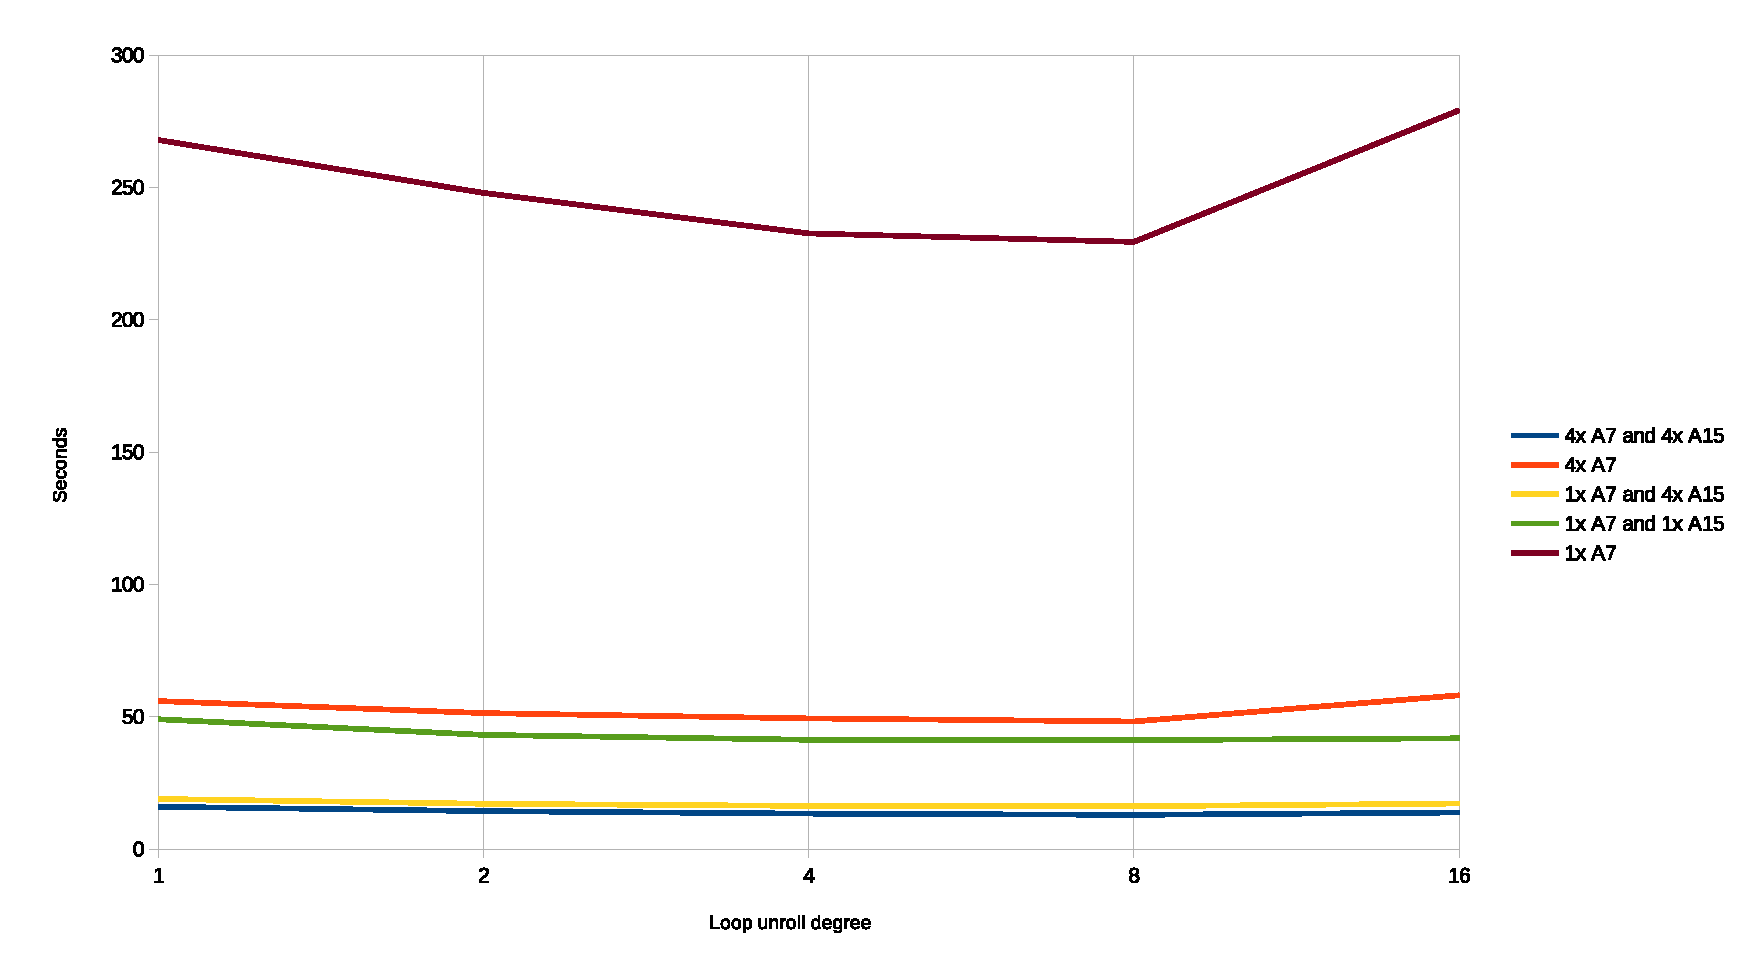
\includegraphics[width=160mm]{fig/loop-unroll-execution-time.eps}
  \caption{Execution time of 2D-Convolution with different degrees of loop unrolling running on different processor configurations. \label{overflow}}
\end{figure}
\begin{table}[H]
  \begin{tabular}{llllll}
    \toprule
    Processor configuration           & \multicolumn{5}{c}{Loop unroll degree} \\
                                      & 1                   & 2         & 4         & 8         & 16 \\
    \midrule
    4x Cortex-A7 and 4x Cortex-A15    & 15.9875             & 14.3006   & 13.3692   & 12.8891   & 13.8013 \\
    4x Cortex-A7                      & 55.8885             & 51.3407   & 49.3267   & 48.1665   & 58.0834 \\
    1x Cortex-A7 and 4x Cortex-A15    & 18.9248             & 17.082    & 16.279    & 16.1658   & 17.1759 \\
    1x Cortex-A7 and 1x Cortex-A15    & 49.0195             & 43.1061   & 41.2549   & 41.1286   & 41.8136 \\
    1x Cortex-A7                      & 267.8882            & 247.8783  & 232.5777  & 229.3884  & 279.1135 \\
    \bottomrule
  \end{tabular}
  \caption{Execution time of 2D-Convolution with different degrees of loop unrolling on different processor configurations. \label{overflow}}
\end{table}

The results show that a loop unroll degree of 8 was optimal for this specific implementation of 2D-Convolution on ODROID-XU3.
This was observed across the results with all tested processor configurations.
Because of this result, the remaining experiments are all run with a loop unroll degree of 8.

As mentioned loop unrolling is limited.
As the size of the loop body increase, the number of instructions for the loop increase.
When the instructions no longer fit in cache, the execution of the loop will be halted to load more instructions each iteration.
There is reason to suspect that this is the main reason for the performance loss at loop unroll degree 16.
In addition data cache misses may also occur more often with larger loop bodies.
In 2D-Convolution there are many read write operations in the loop body.
As the amount of data accessed by each iteration grow, there may occur more cache misses.

\section{Performance}
Even with energy efficiency as the focus, performance data are still interesting.
The data are both useful on their own to observe the power of the system, as well as being a way to compare energy results.
When the energy efficiency of a system is measured, it is important to look at the energy data of the system in light of it's computational power.
A system consuming low amounts of power is not as impressive if it is equally low performing.
These are the results of running 2D-Convolution with 8 as the loop unroll on different processor configurations.

\begin{figure}[H]
  \centering
  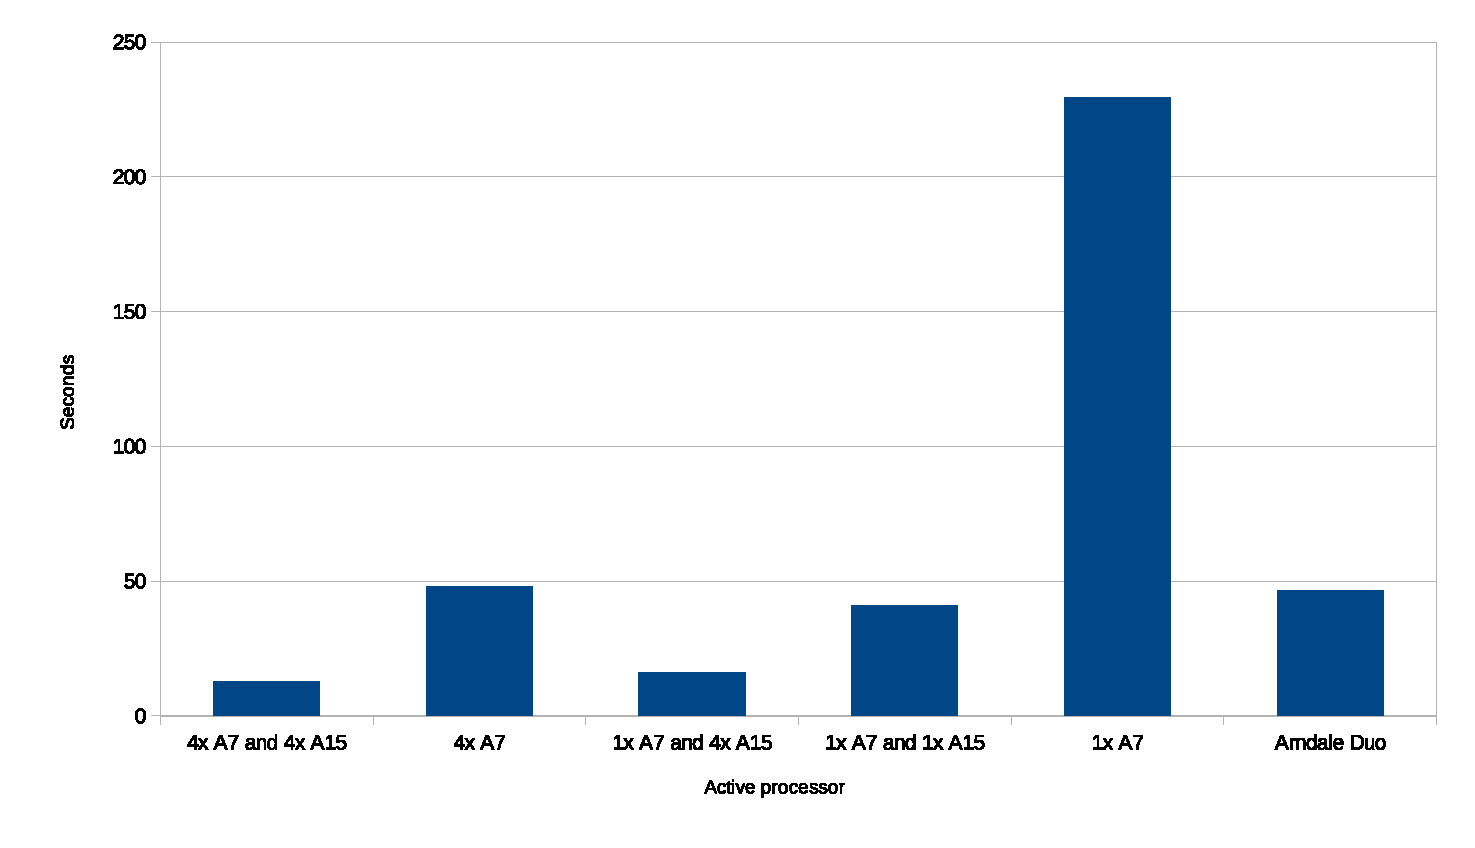
\includegraphics[width=160mm]{fig/execution-time-configurations.eps}
  \caption{Execution time of 2D-Convolution on different processor configurations. All results are from ODROID-XU3 were nothing is specified. The Arndale Board is running at both it's ARM Cortex-A15 cores. The ARM Cortex-A15 cores of the ODROID-XU3 are running at 2.0 GHz, while they are running at 1.7 GHz on the Arndale Board. \label{overflow}}
\end{figure}

\begin{figure}[H]
  \centering
  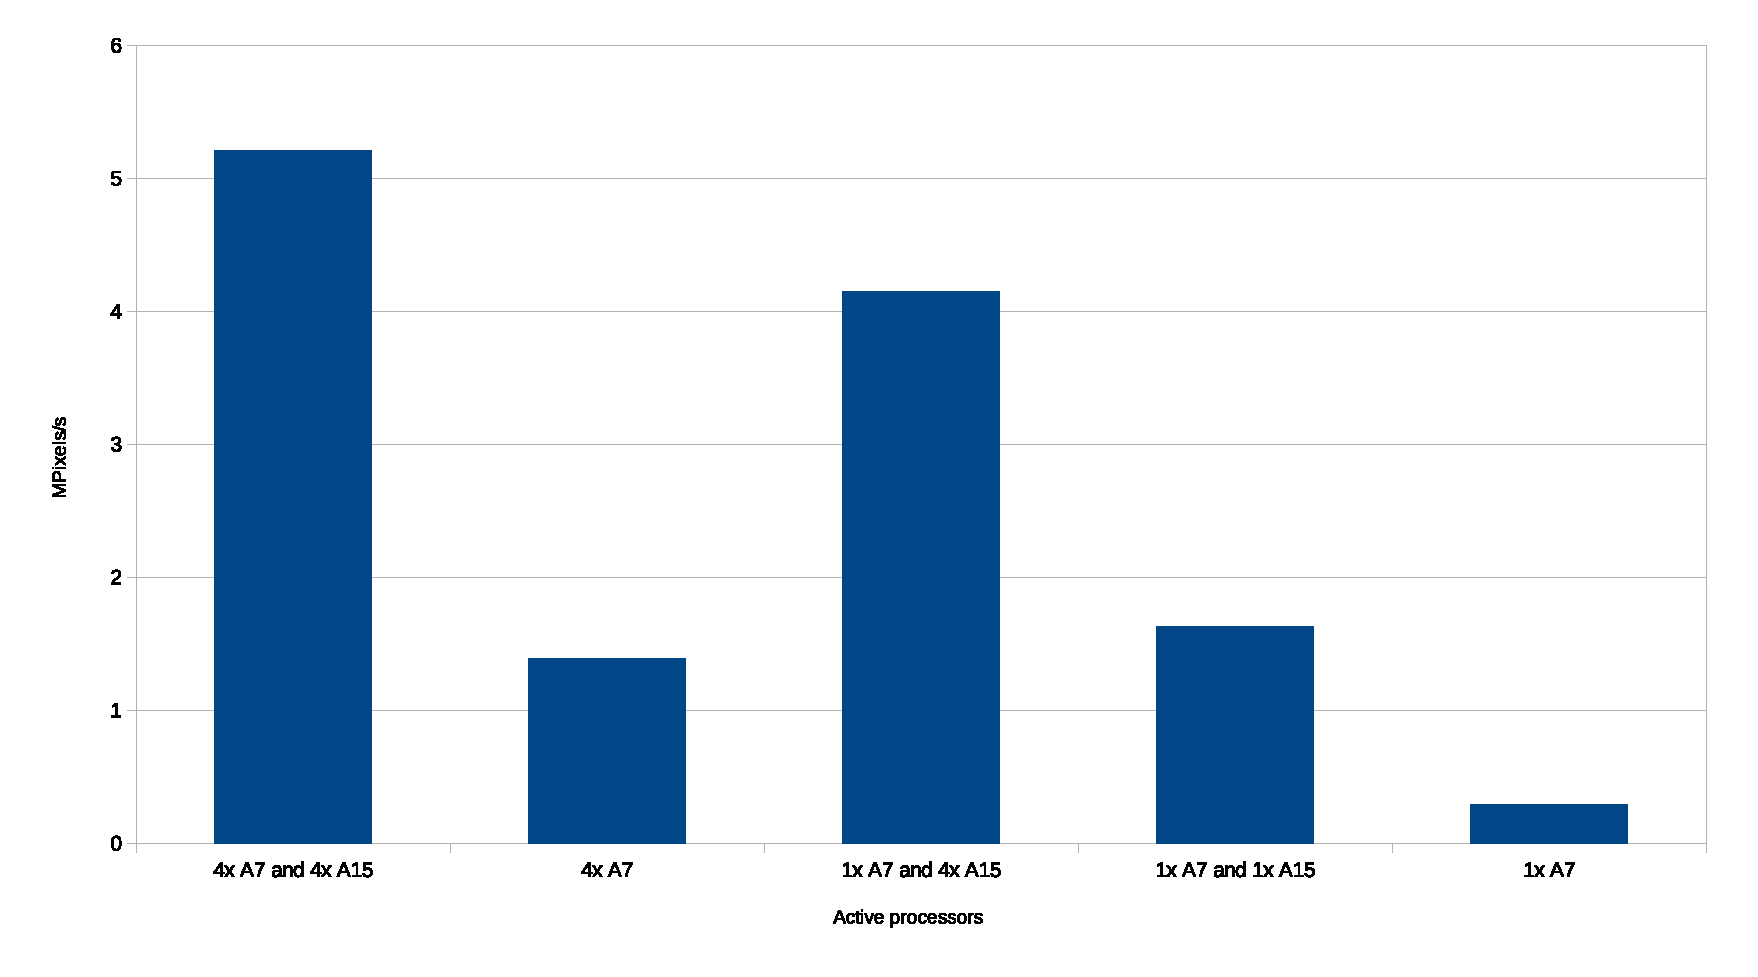
\includegraphics[width=160mm]{fig/mpixelss-configurations.eps}
  \caption{MPixels/s of 2D-Convolution running on different processor configurations. All results are from ODROID-XU3 were nothing is specified. The Arndale Board is running at both it's ARM Cortex-A15 cores. The ARM Cortex-A15 cores of the ODROID-XU3 are running at 2.0 GHz, while they are running at 1.7 GHz on the Arndale Board. \label{overflow}}
\end{figure}

\begin{table}[H]
  \begin{tabular}{llllll}
    \toprule
    Processor configuration           & Execution time (s)  & Performance (MPixels/s) \\
    \midrule
    4x Cortex-A7 and 4x Cortex-A15    & 12.8891             & 5.2066\\
    4x Cortex-A7                      & 48.1665             & 1.3932\\
    1x Cortex-A7 and 4x Cortex-A15    & 16.1658             & 4.1512\\
    1x Cortex-A7 and 1x Cortex-A15    & 41.1286             & 1.6316\\
    1x Cortex-A7                      & 229.3884            & 0.2925\\
    Arndale Board with 2x Cortex-A15    & 46.3942             & 1.4465\\
    \bottomrule
  \end{tabular}
  \caption{Performance of 2D-Convolution with different processor configurations. All results are from ODROID-XU3 were nothing is specified. The ARM Cortex-A15 cores of the ODROID-XU3 are running at 2.0 GHz, while they are running at 1.7 GHz on the Arndale Board. \label{overflow}}
\end{table}

As was to be expected, the large cores perform a lot better than the small ones.
Running the system with all 8 cores powered perform 3.7 times better than the small cores alone.
This is a large performance trade off, but the small cores are still useful if they have a low enough power consumption.

An interesting result here is that adding cores scale sub linearly.
The performance of 4 ARM Cortex-A7 cores and 4 ARM Cortex-A15 is only 3.19 times better than a single ARM Cortex-A7 and a single ARM Cortex-A15.
The reason behind this is likely to be related to memory congestion.
Even though 2D-Convolution is embarrassingly parallel, processor communication is not the only overhead with parallelization.
When running more processors, there are more processors to fight over the memory bandwidth and cause congestion.
This problem is likely to worsen with other more memory intensive problems, and problems with worse cache utilization.
This may lead to some situations where processor configurations, that does not perform well with 2D-Convolution, are well suited.
It would be interesting to explore this in the planned master thesis following this pilot project.

The performance of 4 ARM Cortex-A7 cores is 4.8 times better than a single ARM Cortex-A7.
The small cores seem to scale better than the large ones.
Super linear speedup when adding more cores to a problem, is often a result of each core having its own cache.
More processors with cache give the system as a whole more available cache.
This may also be a result of the other tasks the operating system is running.
With less processing power available, the fraction of time spent running the operating system increase.
Because of this, there is reason to suspect that the small cores don't really scale as well as the results indicate.

The performance experiments run on the older Arndale Board show that it have worse performance with its ARM Cortex-A15 cores than the ODROID-XU3.
The two high power cores on the Arndale board have lower performance than a low power and a high power processor on the ODROID board.
If we assume linear scaling and extrapolate, we see that a quad core ARM Cortex-A15 with Arndale specifications would reach a performance of 2.9 MPixels/s.
On the ODROID-XU3, the similar setup with 4 ARM Cortex-A15 cores and an ARM Cortex-A7 core, had a performance of 4.2 MPixels/s.
The gap between the two is too large to be attributed to the single ARM Cortex-A7.
This performance difference is not surprising, as the Arndales cores run at a lower clock frequency.
They are also paired with slower memory, which may also contribute to the lower performance.

\section{Power measurements}
As described in chapter \ref{setupandmethodology}, separate energy measurements for the different SoC components were gathered during execution of the experiments.
Each of the 4 components value was logged every 200 ms.
The Arndale Board does not feature any on board energy sensors, and measuring power for this board would have to be done for the board as a whole.
As these results would not be comparable to the energy data from ODROID, they were not gathered.
Figure \ref{powerovertime} show the raw energy measurements for a single execution of 2D-Convolution running on all 8 processors.
We can here observe the energy consumption of the program throughout the execution for different components.
The total energy consumption can be calculated from the data.
Observations regarding power usage during different execution stages can also be analyzed.
The same kind of data were gathered for a range of different processor configurations.

\begin{figure}[H]
  \centering
  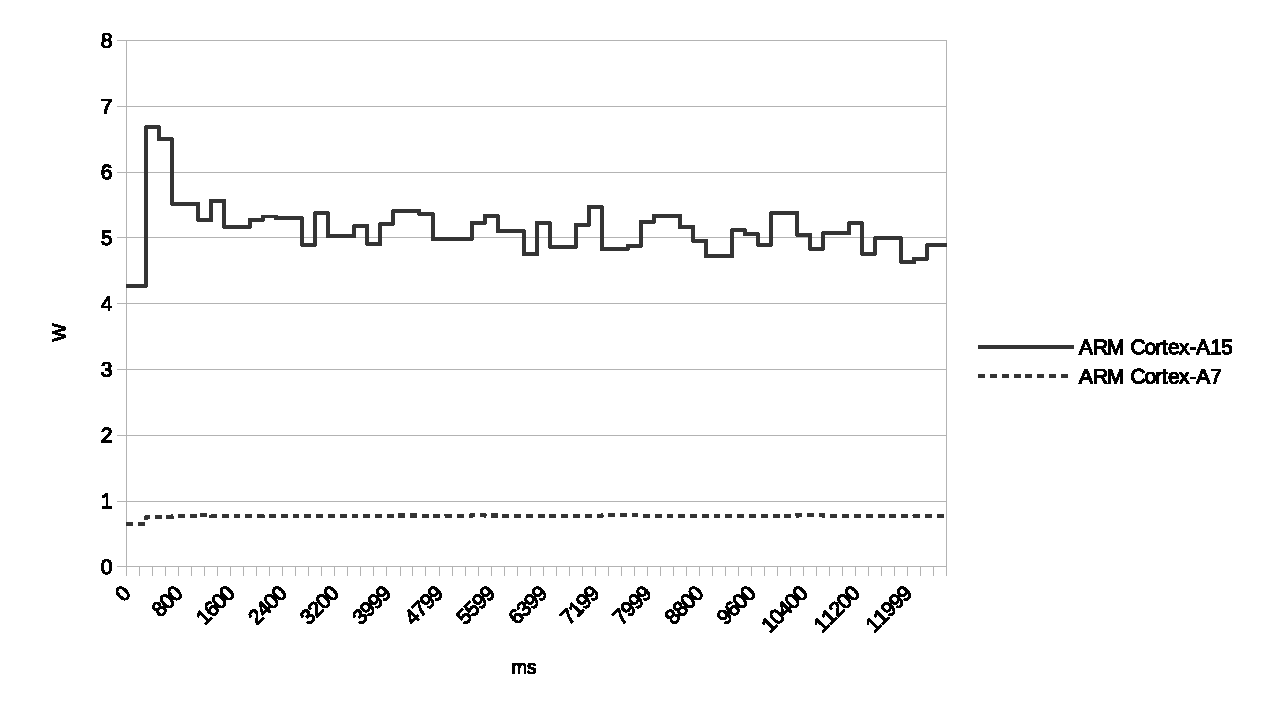
\includegraphics[width=160mm]{fig/power-over-time.eps}
  \caption{Power consumption for the large and small cores during execution of 2D-Convolution with unroll 8x. These results are from a full execution running on all 8 processors. \label{overflow}}\label{powerovertime}
\end{figure}
There is a spike in power consumption on both the small and large cores at the start of the execution.
This spike can be caused by a lot of different reasons.
There is not enough data to know what caused it.
Typical reasons for such spikes are intense operations during initiation of the program, or simply hardware implementations causing a power surge when processor cores are suddenly powered up from idle state.
For the rest of the execution there are variations in power consumption, but the consumption vary around the same general level.

\section{Average power measurements}
Using the data gathered for each component in different processor configurations we can examine their efficiency.
These data are presented in Figure \ref{power-configurations}.
\begin{figure}[H]
  \centering
  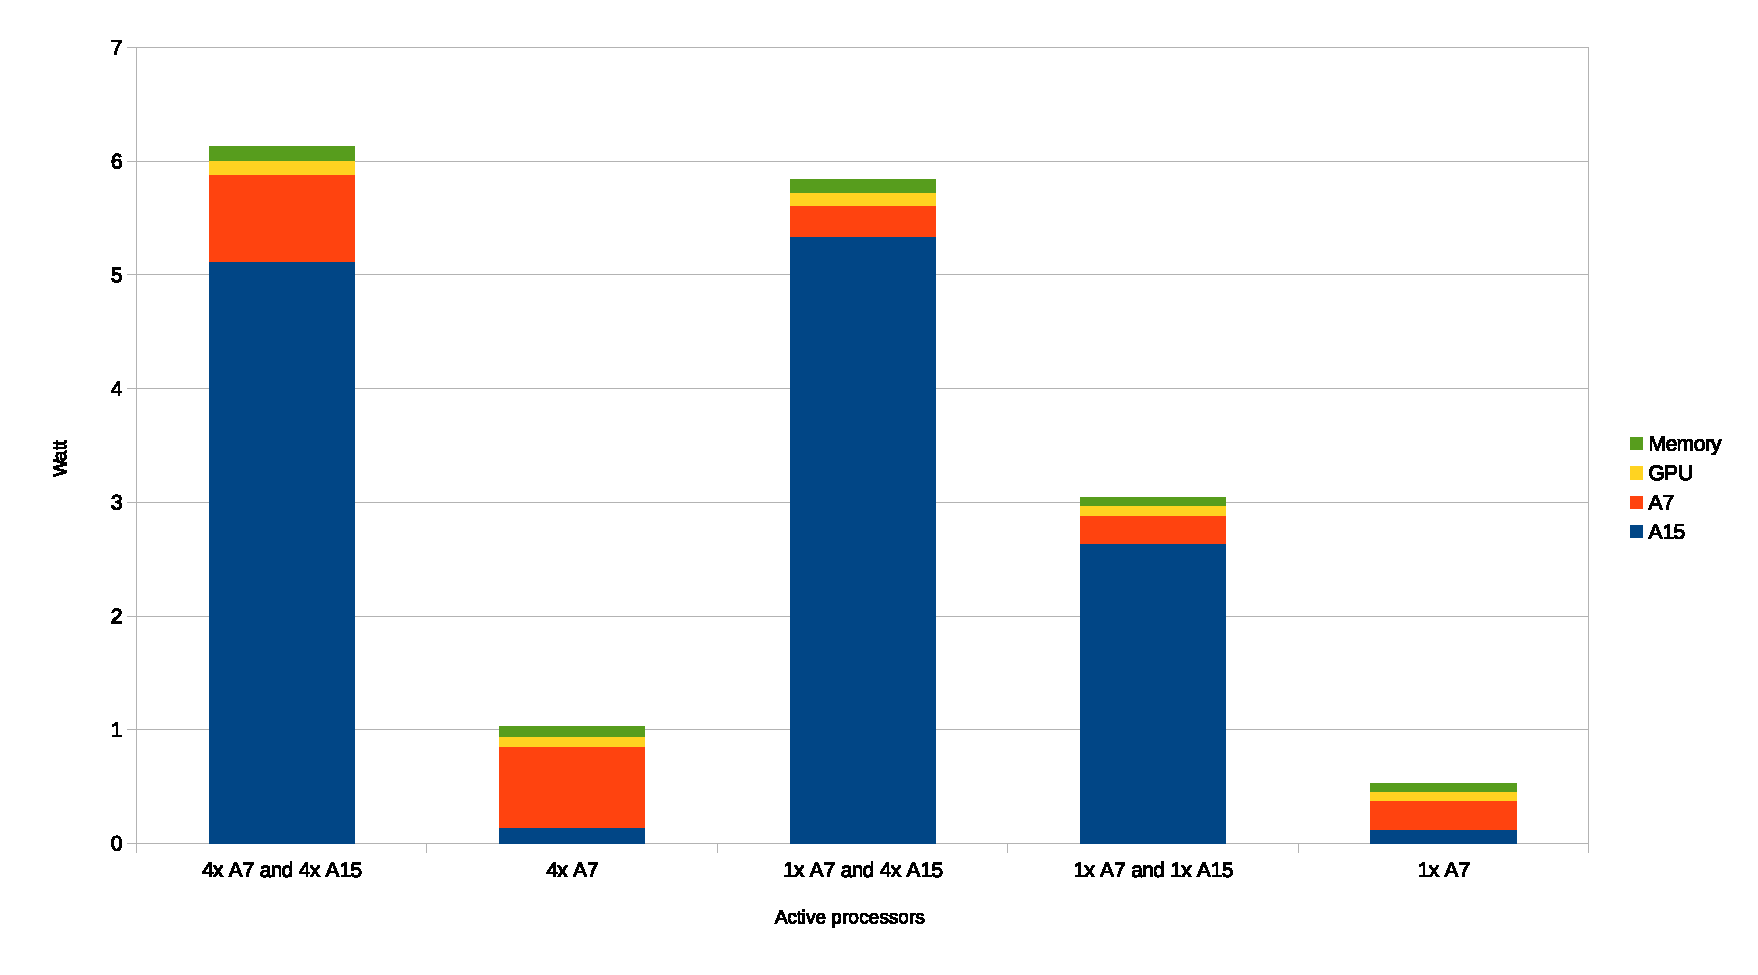
\includegraphics[width=160mm]{fig/power-configurations.eps}
  \caption{Average power consumed per second for different processors configurations running 2D-Convolution. The colors indicate different components, and the full height of each column is the accumulated total for the whole system.\label{overflow}} \label{power-configurations}
\end{figure}

\begin{table}[H]
  \begin{tabular}{llllll}
    \toprule
    Processor configuration         & \multicolumn{5}{c}{Power consumption per second for each component} \\
                                    & Cortex-A15  & Cortex-A7 & Mali-T628 & Memory  & Total \\
    \midrule
    4x Cortex-A7 and 4x Cortex-A15  & 5.1156          & 0.7693        & 0.1206        & 0.1208  & 6.1264 \\
    4x Cortex-A7                    & 0.1362          & 0.7157        & 0.0899        & 0.0817  & 1.0238 \\
    1x Cortex-A7 and 4x Cortex-A15  & 5.3356          & 0.2758        & 0.1161        & 0.1098  & 5.8373 \\
    1x Cortex-A7 and 1x Cortex-A15  & 2.6341          & 0.2540        & 0.0818        & 0.0755  & 3.0456 \\
    1x Cortex-A7                    & 0.1197          & 0.2535        & 0.0813        & 0.0709  & 0.5256 \\
    \bottomrule
  \end{tabular}
  \caption{Execution time of 2D-Convolution with different degrees of loop unrolling on different processor configurations. \label{overflow}}
\end{table}

As expected we see that the power of the ARM Cortex-A7s is a lot lower than the power of the ARM Cortex-A15.
Turning off the power hungry Cortex-A15s reduce the total power to a sixth (0.17).
This is useful for applications running that do not require high performance, and  want to consume low power.
This way of power saving can be increased even more by utilizing only a single Cortex-A7.
This configuration has the lowest power consumption per second, and is useful for standing by, or executing minor calculations while standing by.
Running on only a single Cortex-A7 reduce the power of the system to a tenth (0.10) of that of the fully powered 8 core system.
More than half of this power was used by other components.

In addition to the total power of the system, the results also allow us to analyze the power of each component.
Turning off 3 Cortex-A15 cores only reduce the power to about half (0.51).
Even turning all the Cortex-A15 cores off still leave some power consumed by them.
Because of this power, running the system with only four Cortex-A7 cores still spend 13\% of the total energy on the Cortex-A15 cores, which are not doing any work.
Similarly turning off 3 Cortex-A7 cores only reduce power to a bit more than two thirds (0.35).
These results reveal that the energy for each set of cores are not spent solely on powering the cores themselves, but also some peripheral components related to the cores.
These peripheral components can not be turned partially of, and will consume some power when at least one core is on.
They even consume some power when the cores are all off.
Because of this overhead power from partially powered processors, there rarely occur situations where this is optimal.
The results for such processor configurations will be analyzed further in this project to observe whether or not this is the case here.

\section{Energy consumption measurements}A \label{energyconsumptionmeasurements}
The power usage of the different system components is interesting.
There is however many cases where the system can be put to another task, or shut down, when it is finished.
In such cases it is interesting to observe the total amount of energy consumed completing the task.
In Figure \ref{power-consumed-configurations} the data for each component power usage is multiplied with the execution time.
The data height of each column is the amount of energy consumed.

\begin{figure}[H]
  \centering
  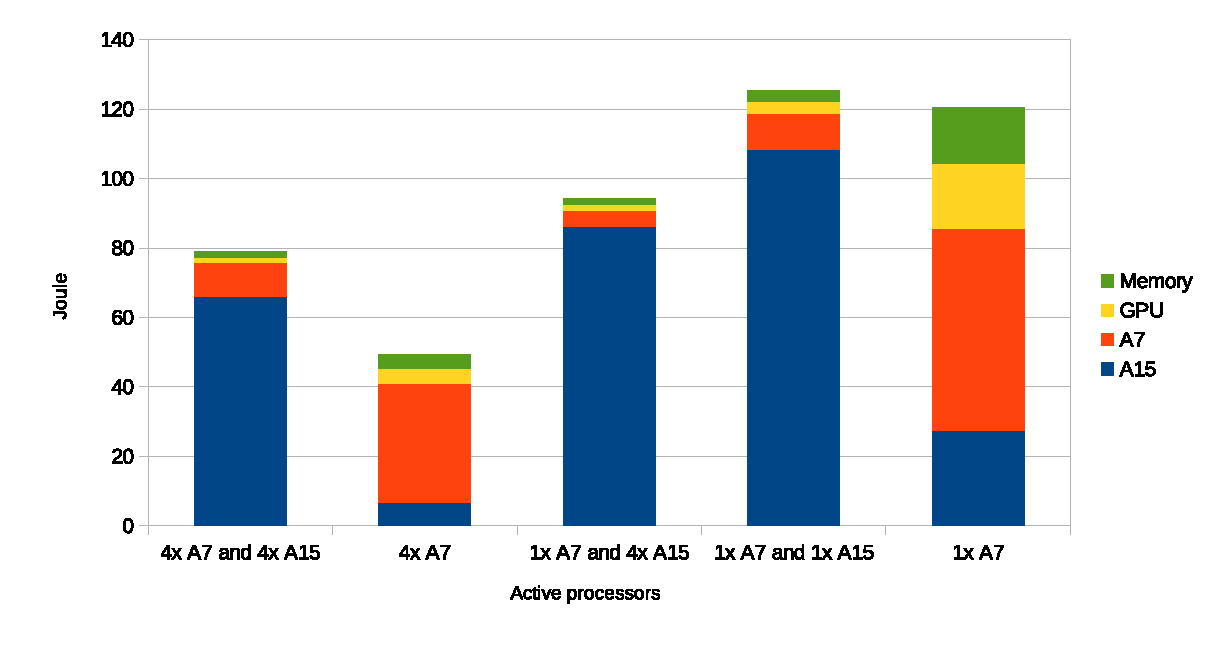
\includegraphics[width=160mm]{fig/power-consumed-configurations.eps}
  \caption{Total energy consumption execution the whole 2D-Convolution program. The colors indicate different components, and the full height of each column is the accumulated total power consumed for the whole system.\label{overflow}} \label {power-consumed-configurations}
\end{figure}

Figure \ref{power-consumed-configurations} show that, even though the fully powered system with all eight processors operating performed better than all the other processor configurations, it is not the best at energy consumption.
The power consumed by a full execution of 2D-Convolution on all 8 processors consume 60\% more power than running it on the 4 Cortex-A7 cores alone.
Running on the more energy efficient, processors cost performance, but it save energy.
This is a trade off that is often observed in energy efficiency.
It vary from application to application what is the preferred property, but it is always an issue of balancing the two.
In section \ref{EDP} the balance point between performance and energy of these experiments are explored in further depth.

Apart from the results for the full eight core system and the 4 small cores, experiments for the other processor configurations were also carried out.
These results however, were not promising.
All the other processor configurations had higher energy consumption than the two first configurations.
They their performance was also worse than the full system, which completed the execution with a lower power consumption.
In other words, they did neither stand out in energy efficiency or performance.
There may exist potential situations with very specific maximum execution times and such, where these configurations may be viable.
They are however not promising candidates for general applications.

\section{Energy Delay Product (EDP) measurements} \label{EDP}
While the energy consumption is a good energy measure in many situations, it is often interesting to compare the energy consumed with it's performance trade off.
As explained in section \ref{energymeasurement} energy delay product measurements can be used to examine this trade off.
These are the energy data from chapter \ref{energyconsumptionmeasurements} multiplied with the execution time of the respective application execution.

\begin{figure}[H]
  \centering
  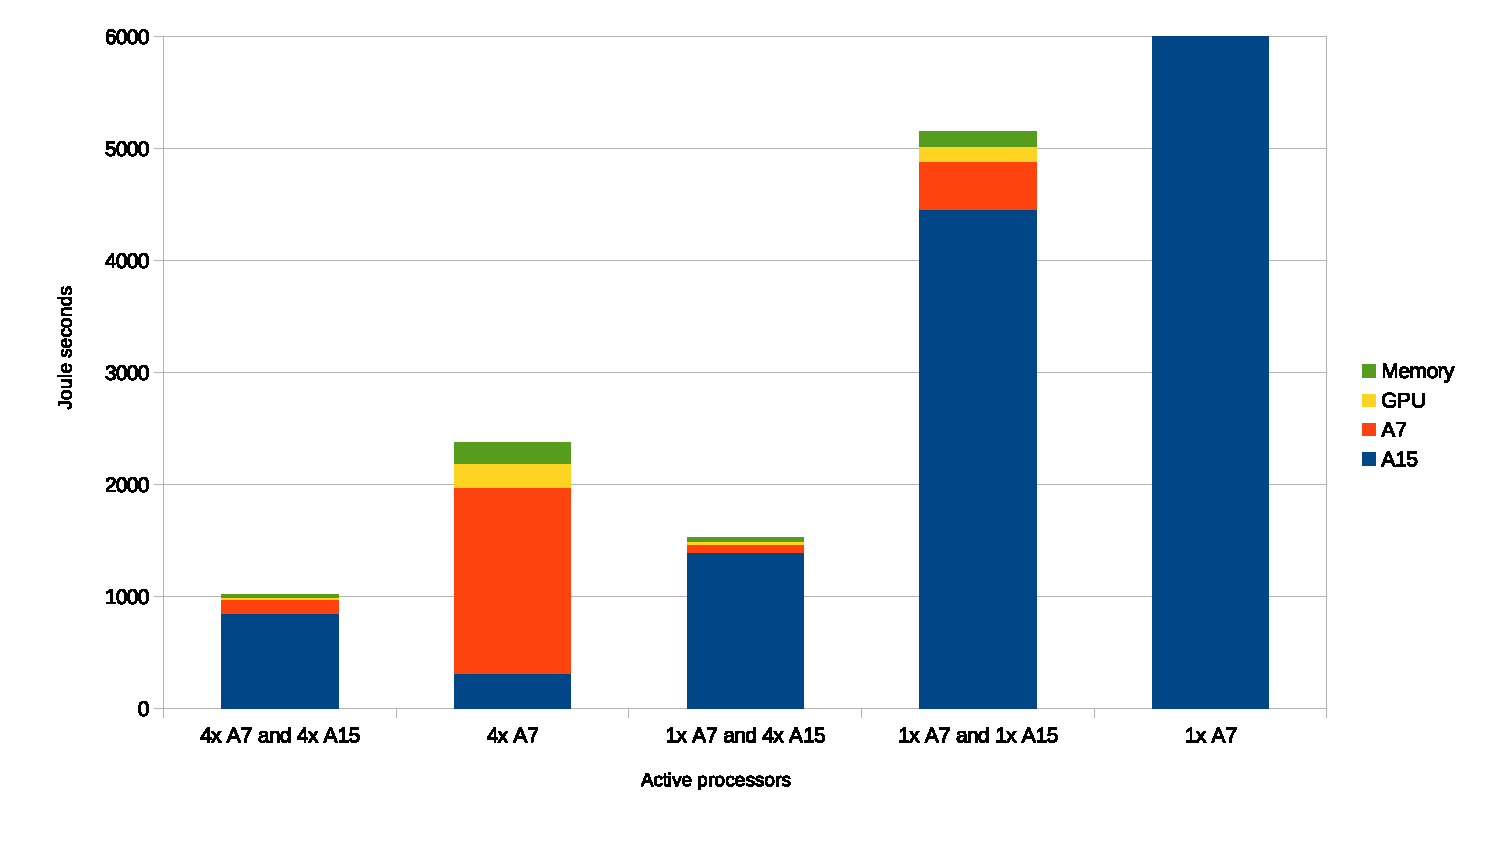
\includegraphics[width=160mm]{fig/EDP-configurations.eps}
  \caption{Energy delay product after execution the whole 2D-Convolution program with different processor configurations. Note that the EDP of the ARM Cortex-A7 goes beyond the scale of the graph with a value of 27658, to allow for better readability. The colors indicate different components, and the full height of each column is the accumulated energy delay product for the whole system.\label{overflow}} \label {EDP-configurations}
\end{figure}

These data clearly show that with energy delay product as out goal, running the fully powered system achieve the best results.
The energy efficiency gain by switching to the smaller and more energy efficient processors, is not worth the performance trade off.
This mean that for applications which require a balanced performance trade off, the more energy efficient Cortex-A7 cores will not be a great alternative in most cases.

It is worth noting that the configuration running on only 1 of the small cores and all the large ones have a decent EDP.
There exist special cases where this processor configuration may be useful.
An example is applications where task dependencies make it inefficient to utilize all processors.
In such a case, the program may run faster by turning off small cores.
It is also obvious that running on the single Cortex-A7 processor, while having the lowest power measurement, is unsuited for any application with performance demand.


% !TEX encoding = UTF-8 Unicode
%!TEX root = thesis.tex
% !TEX spellcheck = en-US
\chapter[Conclution]{Conclution}


% !TEX encoding = UTF-8 Unicode
%!TEX root = thesis.tex
% !TEX spellcheck = en-US
\chapter[Future Work]{Future Work}
These are some suggestions for future work that may build uppon the work in this thesis.

\section{Experiment with heterogenousity}
In this thesis, there have been done experiments with the Exynos 5, which support ARM big.LITTLE.
The heterogen properties of this processor was outside of the scope of this pilot project.
The same applications can be adapted and optimized to explore the potential of this processor architecture.
This is planned for the master thesis following this pilot project.

\section{OmpSs with OpenCL kernels}
A new feature of OmpSs is it's ability to manage OpenCL kernels as tasks.
It is possible to issue OpenCL kernels as OmpSs tasks, and have the task manager assign them to GPUs and CPUs.
This allow for portable code that can run effectivly on a range of different system.
It would be interesting to examine the potency of this way of utilizing the GPU, as it save the programmer from the job of manually tuning the loadbalance between GPU and CPU.

\section{ARMv8-A 64-bit processors}
ARM have created the next generation ARM processors.
They run a new instruction set, with support for both 32- and 64-bit instructions.
Running similar experiments on such a processor would be interesting.

\section{Performance measurement}
In this project, only simple forms of performance measurement was used.
Running the same or similar experiments with access to other performance counters would be interesting.
Cache hit rate and utilization, memory utilization, bus utilization and other counters could help understanding the strengths and weaknesses of the system.


%% !TEX encoding = UTF-8 Unicode
%!TEX root = thesis.tex
% !TEX spellcheck = en-US
%%=========================================
\chapter{Introduction}
The first chapter of a well-structured thesis is always an introduction, setting the scene with background, problem description, objectives, limitations, and then looking ahead to summarize what is in the rest of the report. This is the part that readers look at first---\emph{so make sure it hooks them!}

%%=========================================
\section{Background}
In this section, you should present the problem that you are going to investigate or analyze; why this problem is of interest; what has, so far, been done to solve the problem, and which parts of the problem that remain.

{\color{red}Below, I have set up some headings (subsection titles) without a number. These are included to help you remember to cover the related issues. The headings should be removed in your final print.}
%%=========================================
\subsection*{Problem Formulation}
You should define your problem in a clear an unambiguous way and explain why this is a problem, why it is of interest---and to whom. It is also important to delimit the problem area.
%%=========================================
\subsection*{Literature Survey}
You should here present the main books and articles that treat problems that are similar to what  you are studying. If you,  later in your thesis, describe the ``state of the art'' -- with a detailed literature survey, you may just give a very brief survey here (approx. a quarter of a page). If this is the only literature survey, you need to go into more details. An objective of the literature survey is to show the reader that you are familiar with the main literature within your field of research -- so that you do not ``reinvent the wheel.''


References to literature can be given in two different ways:
\begin{itemize}
\item As an \emph{explicit} reference: It is shown by \citet{lundteigen08} and partly also by \citet{rausand14}  that \ldots.
\item As an \emph{implicit} reference: It is shown \citep[e.g., see][Chap. 4]{rausand04} that \ldots.
\end{itemize}
In the example above, we have used ``author-year'' references, which is the preferred format. 
\begin{remark}
Following agreement with your supervisor, you may also refer by numbers, for example,  [1]. To do this, open the file \texttt{ramsstyle.sty} and  comment out (by \%) the command \texttt{$\backslash$usepackage\{natbib\}} and un-comment the corresponding command \texttt{$\backslash$usepackage[numbers]\{natbib\}}.\footnote{Notice the strange way we have to write the ``backslash'' in the text. This is because the ``backslash'' is a command in \LaTeX.}
\end{remark}
 You may include a link to the Internet in the text or in a footnote by using a command like: \url{http://www.ntnu.edu/ross}. 

When you refer to the scientific literature, you should always write in \emph{present} tense. Example: \citet{rausand04} show that \ldots.

\begin{remark}
Hyperlinks are included by the command \texttt{$\backslash$usepackage\{hyperref}\} in \texttt{ramsstyle.sty}. If you feel that the hyperlinks are disturbing when you enter the text, or want to avoid the hyperlinks in printed text, you may either comment out or edit this command in \texttt{ramsstyle.sty}.
\end{remark}
%%=========================================
\subsection*{What Remains to be Done?}
After you have defined and delimited your problem -- and presented the relevant results found in the literature within this field, you should sum up which parts of the problem that remain to be solved.
%%=========================================
\section{Objectives}
The main objectives of this Master's project are
\begin{enumerate}
\item This is the first objective
\item This is the second objective
\item This is the third objective
\item More objectives
\end{enumerate}

The objectives shall be written as \emph{fundamental objectives} telling what to do and not \emph{means objectives} telling how to do it.

All objectives shall be stated such that we, after having read the thesis, can see whether or not you have met the objective. ``To become familiar with \ldots'' is therefore not a suitable objective.

%%=========================================
\section{Limitations}
In this section you describe the limitations of your study. These may be related to the study object (physical limitations, operational limitations), to the environmental and operational conditions, to the thoroughness of the analysis, and so on.
%%=========================================
\section{Approach}
Here you should describe the (scientific) approach that you will use to solve the problem and meet your objectives. You should specify the approach for each objective.

If there are any ethical problems related to your approach, these should be highlighted and discussed.
%%=========================================
\section{Structure of the Report}
The rest of the report is organized as follows. Chapter 2 gives an introduction to \ldots

\begin{remark}
Notice that chapter and section headings shall be written in lowercase, but that all main words should start with a capital letter.
\end{remark}


The report should be no longer than \underline{60 pages} in this format (+ the CV).
%% !TEX encoding = UTF-8 Unicode
%!TEX root = thesis.tex
% !TEX spellcheck = en-US
%%=========================================
\chapter[Equations, etc]{Equations, Figures, and Tables}
The content of Chapter 2 will vary with the topic of your thesis. This chapter only gives guidance to some technical aspects of \LaTeX.
 
\begin{remark}
If you want a shorter chapter or section title to appear in the Table of Contents and in the headings of the chapter, you just include the short title in square brackets before the title of the chapter/section. Example: \begin{verbatim}\section[Short Title]{Long Title}\end{verbatim}.
\end{remark}

%%=========================================
\section{Simple Equations}
Mathematical symbols and equations can written in the text as $\lambda$, $F(t)$, or even $F(t)=\int_0^t \exp(-\lambda x)\,dx$, or as displayed equations
\begin{equation}
F(t)=\int_0^t \exp(-\lambda x)\,dx
\label{eq1}
\end{equation}


The displayed equations are automatically given equation numbers -- here (\ref{eq1}) since this is the first equation in Chapter 2. Note that you can refer to the equation by referring to the ``label'' you specified as part of the equation environment.

You can also include equations without numbers:
\begin{equation*}
F(t)=\sum_{i=1}^n \binom{n}{i}\sin(i\cdot t)
\end{equation*}

%%=========================================
\subsection*{More Advanced Formulas}
Long formulas that cannot fit into a single line can be written by using the environment \texttt{align} as
\begin{align}
F(t)&= \sum_{i=1}^n \sin(t^{n-1}) - \sum_{i=1}^n \binom{n}{i}\sin(i\cdot t) \\
      & + \int_0^\infty n^{-x} e^{-\lambda x^t}\,dt
\end{align}

In some cases, you need to write ordinary letters inside the equations. You should then use the commands 
\begin{verbatim}
\textrm  and/or \mathrm
\end{verbatim}
The first command returns the normal text font and will be scaled automatically, while the second command will be scaled according to the use.
\begin{equation*}
\textrm{MTTF}= \int_0^\infty R_\mathrm{avg}(t)\,dt
\end{equation*}



Please consult the \LaTeX\ documentation for further details about mathematics in \LaTeX.
%%=========================================
\section*{Definitions}
If you want to include a definition of a term/concept in the text, I have made the following macro (see in \texttt{ramsstyle.sty}):
\begin{defin}
\textbf{Reliability}: The ability of an item to perform a required function under stated environmental and operational conditions and for a stated period of time.\newline
\end{defin}
When text is following directly after the definition, it may sometimes be necessary to end the definition text by the command
\begin{verbatim}
\newline
\end{verbatim}
I have not included this in the definition of the \texttt{defin} environment to avoid too much space when there is not a text-block following the definition.
%%=========================================
\section{Including Figures}
If you use pdf\LaTeX\ (as recommended), all the figures must be in pdf, png, or jpg format. We recommend you to use the pdf format.  Please place the figure files in the directory \textbf{fig}. Figures are included by the command shown for Figure~\ref{fig1}. Please notice the ``path'' to the figure file written by a \emph{forward} slash (/). You should not include the format of the figure file (pdg, png, or jpg) -- just write the ``name'' of the figure. 
\begin{figure}
\centering

\includegraphics[scale=0.6,angle=15]{fig/NTNU}
\caption{This is the logo of NTNU (rotated 15 degrees).}
\label{fig1}
\end{figure}

Each figure should include a unique \emph{label} as shown in the command for Figure~\ref{fig1}. You can then refer to the figure by the \emph{ref} command.
Notice that you can scale the size of the figure by the option \texttt{scale=k}. You may also define a specific width or height of the figure by replacing the \texttt{scale} options by \texttt{width=k} or \texttt{height=k}. The factor \texttt{k} can here be specified in mm, cm, pc, and many other length measures. You may also give \texttt{k} as a fraction of the width of the text or of the height of the text, for example, \texttt{width=0.45$\backslash$textwidth}. If you later change the margins of the text, the figure width will change accordingly. As illustrated in Figure~\ref{fig1}, you may also rotate the figure -- and also do many other things (please check the documentation of the package \texttt{graphicx} -- it is available on your computer, or you may find it on the Internet).

In \LaTeX\ all figures are floating objects and will normally be placed at the top of a page. This is the standard option in all scientific reports. If you insist on placing the figure exactly where you declare the figure, you may include the command \texttt{[h]} (here) immediately after $\backslash$\texttt{begin\{figure\}}. If you will force the figure to be located either at the top or bottom of the page, you may alternatively use  \texttt{[t]} or \texttt{[b]}. For more options, check the documentation.

Large figures may be included as a \emph{sidewaysfigure} as shown in Figure~\ref{fig2}:\footnote{You can use a similar command for large tables.}
\begin{sidewaysfigure}
\centering

\includegraphics[scale=1.8]{fig/NTNU}
\caption{This is the logo of NTNU.}
\label{fig2}
\end{sidewaysfigure}

%%=========================================
\section{Including Tables}
\LaTeX\ has a lot of different options to include tables. Only one of them is illustrated here.

\begin{table}
	\centering\small
	\caption{The degree of newness of technology.}
	\label{tab1}
		\begin{tabular*}{\textwidth}{@{\extracolsep{\fill}}lccc}
			\toprule
			  &\multicolumn{3}{c}{Level of technology maturity}\\
  \cmidrule{2-4}
			Experience with the		   &  & Limited field history or not & New or \\
              operating  condition  & Proven &  used by company/user & unproven \\
        
			\midrule
			  Previous experience & 1 & 2 & 3 \\
		          No experience by company/user & 2 & 3 & 4 \\
		          No industry experience & 3 & 4 & 4 \\
			\bottomrule
		\end{tabular*}
\end{table}

\begin{remark}
Notice that figure captions (Figure text) shall be located \emph{below} the figure -- and that the caption of tables shall be \emph{above} the table. This is done by placing the $\backslash$\texttt{caption} command beneath the command $\backslash$\texttt{includegraphics} for figures, and above the command $\backslash$\texttt{begin\{tabular*\}} for tables.
\end{remark}
%%=========================================
\section{Copying Figures and Tables}
In some cases, it may be relevant to include figures and tables from from other publications in your report. This can be a direct copy or that you retype the table or redraw the figure. In both cases, you should include a reference to the source in the figure or table caption. The caption might then be written as: \textsl{Figure/Table xx: The caption text is coming here \citep{rausand04}.}

In other cases, you get the idea from a figure or table in a publication, but modify the figure/table to fit your purpose. If the change is significant, your caption should have the following format: \textsl{Figure/Table xx: The caption text is coming here \citep[adapted from][]{rausand04}.}

%%=========================================
\section{References to Figures and Tables}
Remember that all figures and tables shall be referred to and explained/discussed in the text. If a figure/table is not referred to in the text, it shall be deleted from the report.
%%=========================================
\section{A Word About Font-encoding}
When you press a button (or a combination of buttons) on your keyboard, this is represented in your computer according to the \emph{font-encoding} that has been set up. A wide range of font-encodings are available and it may be difficult to choose the ``best'' one. In the template, I have set up a font-encoding called UTF-8 which is a modern and very comprehensive encoding and is expected to be the standard encoding in the future. Before you start using this template, you should open the Preferences ->Editor dialogue in TeXworks (or TeXShop if you use a Mac) and check that encoding UTF-8 has been specified. 

If you use only numbers and letters used in standard English text, it is not very important which encoding you are using, but if you write the Norwegian letters æ, ø, å and accented letters, such as é and ä, you may run into problems if you use different encodings. Please be careful if you cut and paste text from other word-processors or editors into your \LaTeX\ file!

\subsubsection*{Warning}
If you (accidentally) open your file in another editor and this editor is set up with another font-encoding, your non-standard letters will likely come out wrong. If you do this, and detect the error, be sure \emph{not} to save your file in this editor!!

This is not a specific \LaTeX\ problem. You will run into the same problem with all editors and word-processors -- and it is of special importance if you use computers with different platforms (Windows, OSX, Linux).

%%=========================================
\section{Plagiarism}
Plagiarism is defined as ``use, without giving reasonable and appropriate credit to or acknowledging the author or source, of another person's original work, whether such work is made up of code, formulas, ideas, language, research, strategies, writing or other form'', and is a very serious issue in all academic work. You should adhere to the following rules:
\begin{itemize}
\item Give proper references to all the sources you are using as a basis for your work. The references should be give to the original work and not to newer sources that mention the original sources.
\item You may copy paragraphs up to 50 words when you include a proper reference. In doing so, you should place the copied text in inverted commas (i.e., ``Copied text follows \ldots''). Another option is to write the copied text as a quotation, for example:
\begin{quote}
Birnbaum's measure of reliability importance of component $i$ at time $t$ is equal to the probability that the system is in such a state at time $t$ that component $i$ is critical for the system.\newline \mbox{} \hfill \citet{rausand04}
\end{quote}
\end{itemize}




%% !TEX encoding = UTF-8 Unicode
%!TEX root = thesis.tex
% !TEX spellcheck = en-US
%%=========================================
\chapter[Summary]{Summary and Recommendations for Further Work}
%%This is the last chapter
In this final chapter you should sum up what you have done and which results you have got. You should also discuss your findings, and give recommendations for further work.

%%=========================================
\section{Summary and Conclusions}
Here, you present a brief summary of your work and list the main results you have got. You should give comments to each of the objectives in Chapter 1 and state whether or not you have met the objective. If you have not met the objective, you should explain why (e.g., data not available, too difficult).

This section is similar to the Summary and Conclusions in the beginning of your report, but more detailed---referring to the the various sections in the report.

%%=========================================
\section{Discussion}
Here, you may discuss your findings, their strengths and limitations.
%%=========================================
\section{Recommendations for Further Work}
You should give recommendations to possible extensions to your work. The recommendations should be as specific as possible, preferably with an objective and an indication of a possible approach.

The recommendations may be classified as:
\begin{itemize}
\item Short-term
\item Medium-term
\item Long-term
\end{itemize}
% Include more chapters as required.
%%=========================================
\appendix
% !TEX encoding = UTF-8 Unicode
%!TEX root = thesis.tex
% !TEX spellcheck = en-US
%%=========================================

\chapter{Implementation}

%%=========================================
\section{Introduction}

%%=========================================
\subsection{Program 1}

% Include more appendices as required.
%%=========================================
\bibliographystyle{unsrt}
\addcontentsline{toc}{chapter}{\bibname}
\bibliography{refs}{}
%%=========================================

\end{document}
